\documentclass[aspectratio=169]{beamer}

% Шрифты и локализация
\usepackage{fontspec}
\setmainfont{Times New Roman}
\setsansfont{Arial}
\setmonofont{Courier New}
\usepackage[russian]{babel}

% Изображения
\usepackage{graphicx}
\usepackage{ragged2e}
\usepackage{tikz}

% Оформление слайдов
\setbeamertemplate{navigation symbols}{} % Убираем навигационные символы
\setbeamertemplate{footline}{} % Убираем нижнюю панель
\setbeamertemplate{headline}{} % Чистый заголовок

% Цветовая палитра
\usecolortheme{spruce}
\useinnertheme{circles}

% Стиль заголовков
\setbeamerfont{frametitle}{size=\large, series=\bfseries}

% Титульная информация
\institute{МИНИСТЕРСТВО ОБРАЗОВАНИЯ И НАУКИ РФ\\
Федеральное государственное бюджетное образовательное учреждение высшего образования «Белгородский государственный технологический университет им. В.Г. Шухова»}
\title{Разработка front-end Web–приложения – учебной среды с чатами и AI-анализом кода лабораторных работ}
\author{Автор работы: Бондаренко Сергей Владимирович\\[0.5em]
Направление подготовки: 09.03.04 «ПРОГРАММНАЯ ИНЖЕНЕРИЯ»\\[0.5em]
Руководитель: Мельников Антон Борисович}

\begin{document}

\begin{frame}[plain]
\vspace{1em}
\centering
{\small
МИНИСТЕРСТВО ОБРАЗОВАНИЯ И НАУКИ РФ \\
Федеральное государственное бюджетное образовательное учреждение высшего образования \\
\textbf{«Белгородский государственный технологический университет им. В.Г. Шухова»} \\
\vspace{0.25em}
Кафедра программного обеспечения вычислительной техники и автоматизированных систем
}

\vspace{1em}

{\large \textbf{ВЫПУСКНАЯ КВАЛИФИКАЦИОННАЯ РАБОТА}}

\vspace{1em}

\begin{minipage}{0.95\textwidth}
\centering
«\textbf{Разработка front-end Web-приложения – учебной среды с чатами и AI-анализом кода лабораторных работ}»
\end{minipage}

\vspace{1em}
{\RaggedRight
\begin{minipage}{0.95\textwidth}
\footnotesize
\textbf{Автор работы:} Бондаренко Сергей Владимирович \\[0.25em]
\textbf{Направление подготовки:} 09.03.04 «Программная инженерия» \\[0.25em]
\textbf{Руководитель:} Мельников Антон Борисович, руководитель департамента автоматизации бизнеса ООО «Технологии надежности»
\end{minipage}
}
\end{frame}


% Пример первого слайда
\begin{frame}{Цель и задачи}
\textbf{Цель:} повысить эффективность и облегчить работы преподавателей и обучения студентов через создание front-end части Web-приложения для управления учебным процессом, общения и автоматической проверки заданий.

\vspace{0.5em}
\textbf{Задачи:}
\begin{enumerate}
	\item Провести анализ существующих образовательных решений.
	\item Определить архитектуру и технологический стек.
	\item Разработать пользовательский интерфейс.
	\item Реализовать модули для управления учебными структурами, заданиями и системой общения.
	\item Интегрировать модуль автоматической проверки решений с использованием ИИ.
	\item Провести тестирование бизнес-логики приложения.
\end{enumerate}
\end{frame}

\begin{frame}{Анализ существующих образовательных решений}
\small
\justifying
Проблема заключается в том, что Google Classroom, Microsoft Teams for Education и Moodle решают задачи управления заданиями. VK, Telegram и Viber предназначены только для общения. А CodeSignal и Codility реализуют исключительно AI-анализ кода.

\vspace{0.8em}

Из-за разделения функций между разными сервисами преподаватели и студенты вынуждены постоянно переключаться между несколькими приложениями, что создаёт неудобства и снижает эффективность работы.

\vspace{1em}

\centering
\begin{tabular}{lccc}
\hline
\textbf{Аналоги/Функции} & Система заданий & Общение & AI-анализ \\
\hline
Google Classroom & + & -- & -- \\
MS Teams         & + & +  & -- \\
Moodle           & + & -- & -- \\
CodeSignal       & -- & -- & +  \\
Codility         & -- & -- & +  \\
\hline
\end{tabular}
\end{frame}

\begin{frame}{Стек технологий}

\centering

\includegraphics[height=1.6cm]{static/nextjs-logo.png} \hspace{1cm}

\includegraphics[height=1.6cm]{static/react-logo.png} \hspace{1cm}

\includegraphics[height=1.6cm]{static/typescript-logo.png}

\vspace{1.5em}
\small
\begin{itemize}
  \item \textbf{Next.js} — используется для серверного рендеринга (SSR), маршрутизации и повышения производительности клиентского приложения.
  \item \textbf{React} — обеспечивает декларативный подход к построению компонентного пользовательского интерфейса.
  \item \textbf{TypeScript} — добавляет статическую типизацию, улучшает читаемость и сопровождаемость кода.
\end{itemize}
\end{frame}

\begin{frame}{Архитектура Web-приложения}
\begin{columns}
    \begin{column}{0.45\textwidth}
        \centering
        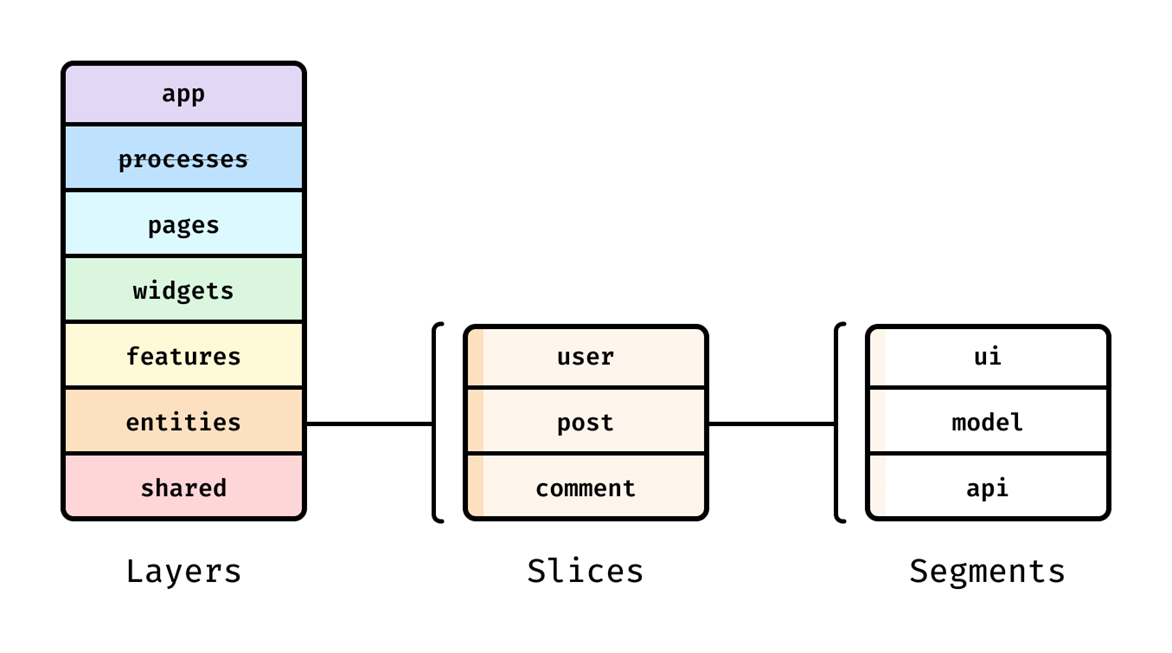
\includegraphics[width=0.8\linewidth]{static/fsd-diagram.png} \\
        \small FSD-архитектура
    \end{column}
    \begin{column}{0.45\textwidth}
        \centering
        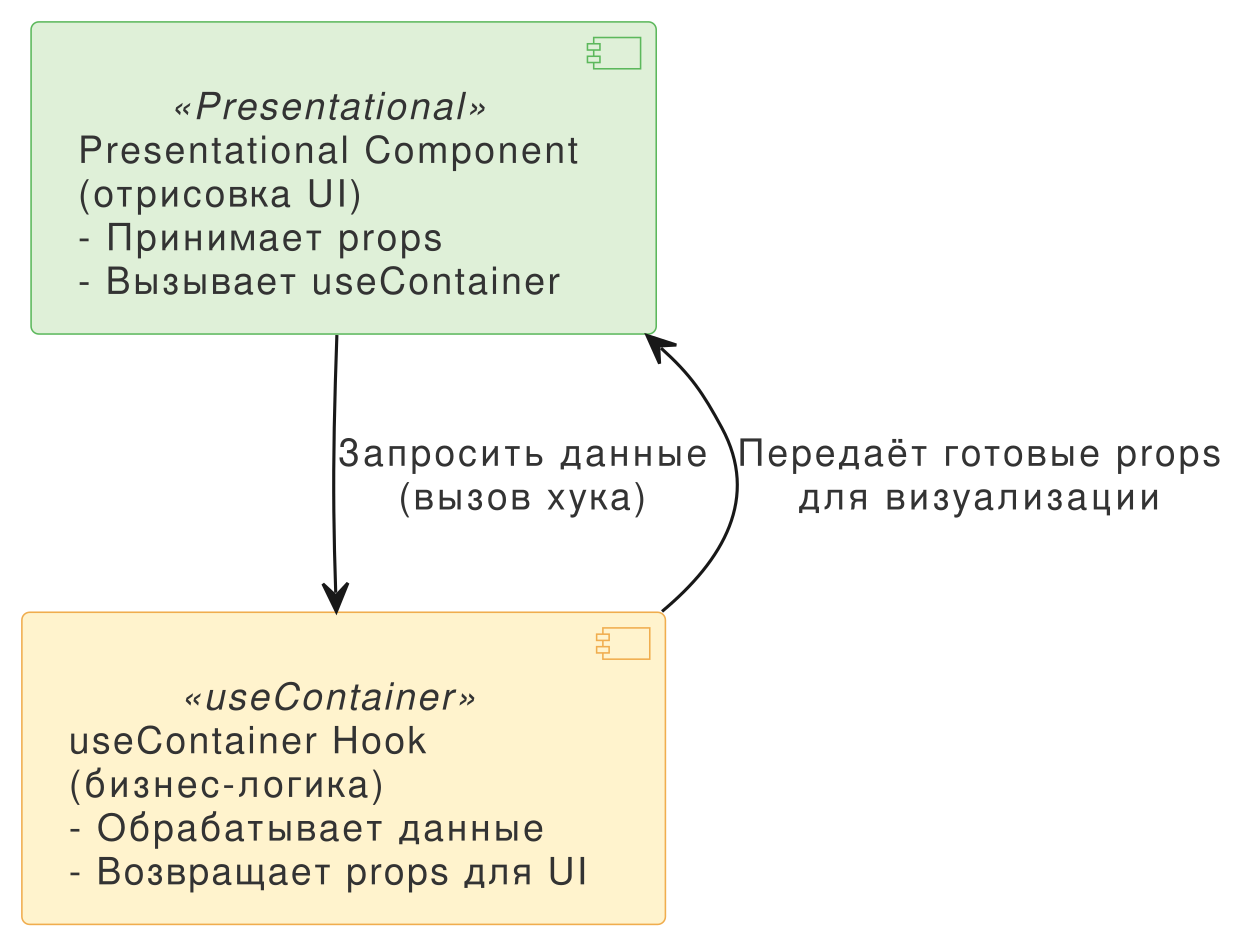
\includegraphics[width=0.8\linewidth]{static/container-presentational.png} \\
        \small Контейнерно-презентационный подход
    \end{column}
\end{columns}

\vspace{0.5em}

\small
\begin{itemize}
  \item \textbf{Feature-Sliced Design (FSD)} — архитектурный подход, основанный на разделении приложения на функциональные срезы и уровни, что упрощает масштабирование и сопровождение.
  \item \textbf{Container/Presentational Components} — паттерн, разделяющий компоненты на логические и визуальные.
\end{itemize}

\end{frame}

\begin{frame}{Модуль аутентификации и авторизации}
\small

\begin{columns}
    \begin{column}{0.5\textwidth}
        \centering
        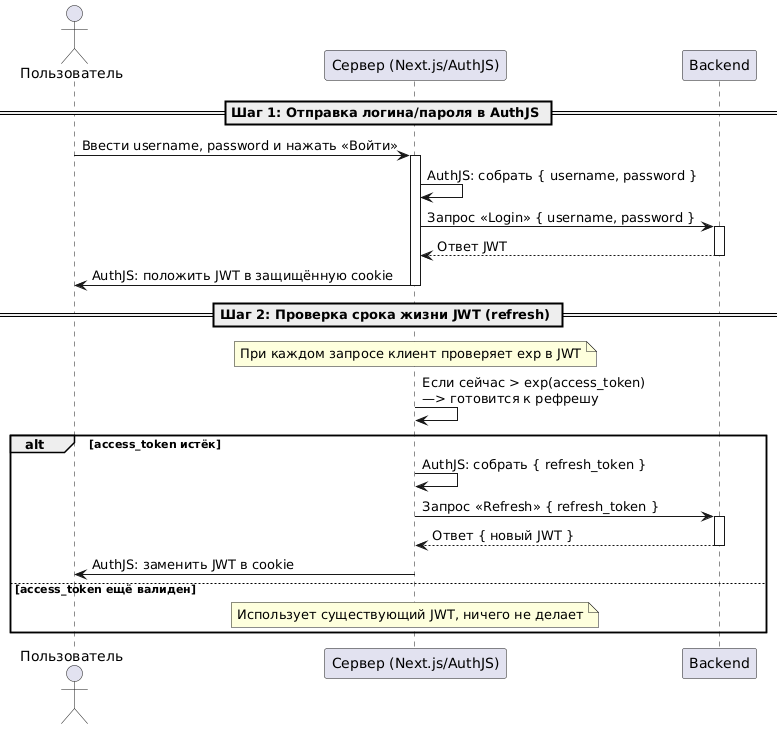
\includegraphics[width=0.95\linewidth]{static/AuthRefresh.png} \\
        \small Диаграмма авторизации и аутентификации
    \end{column}
    \begin{column}{0.5\textwidth}
        \centering
        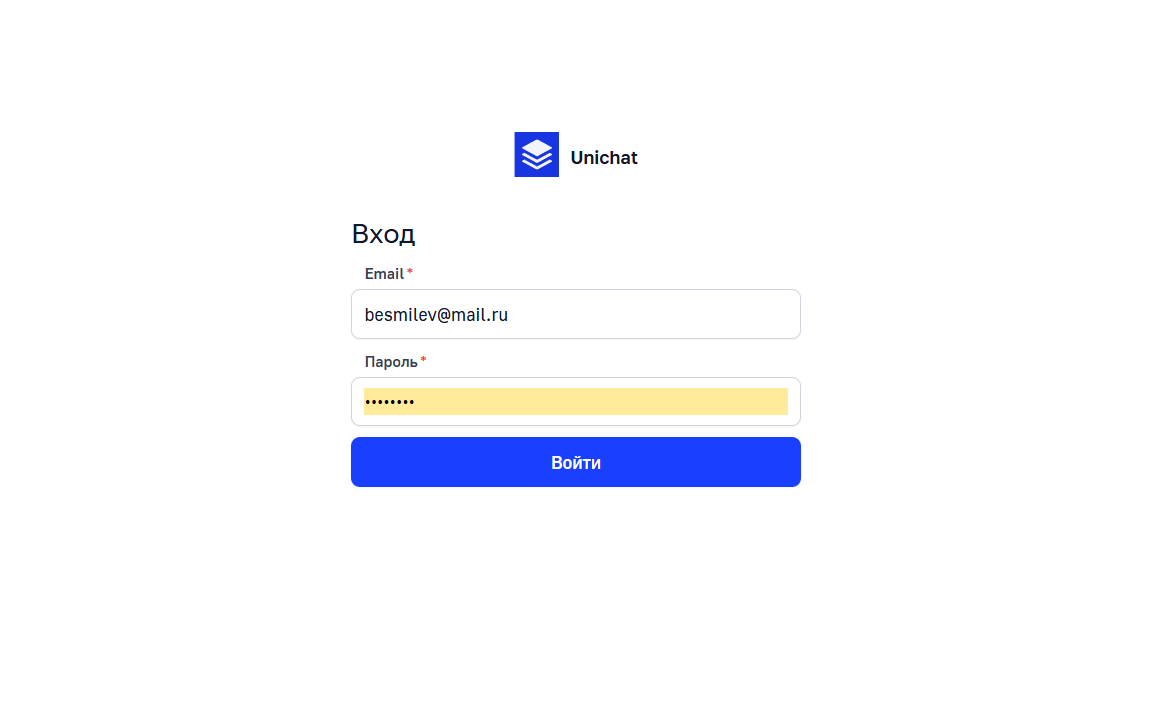
\includegraphics[width=0.95\linewidth]{static/LoginPage.png} \\
        \small Интерфейс входа
    \end{column}
\end{columns}
\end{frame}

\begin{frame}{Взаимодействие администратора с web-приложением}
    \centering
    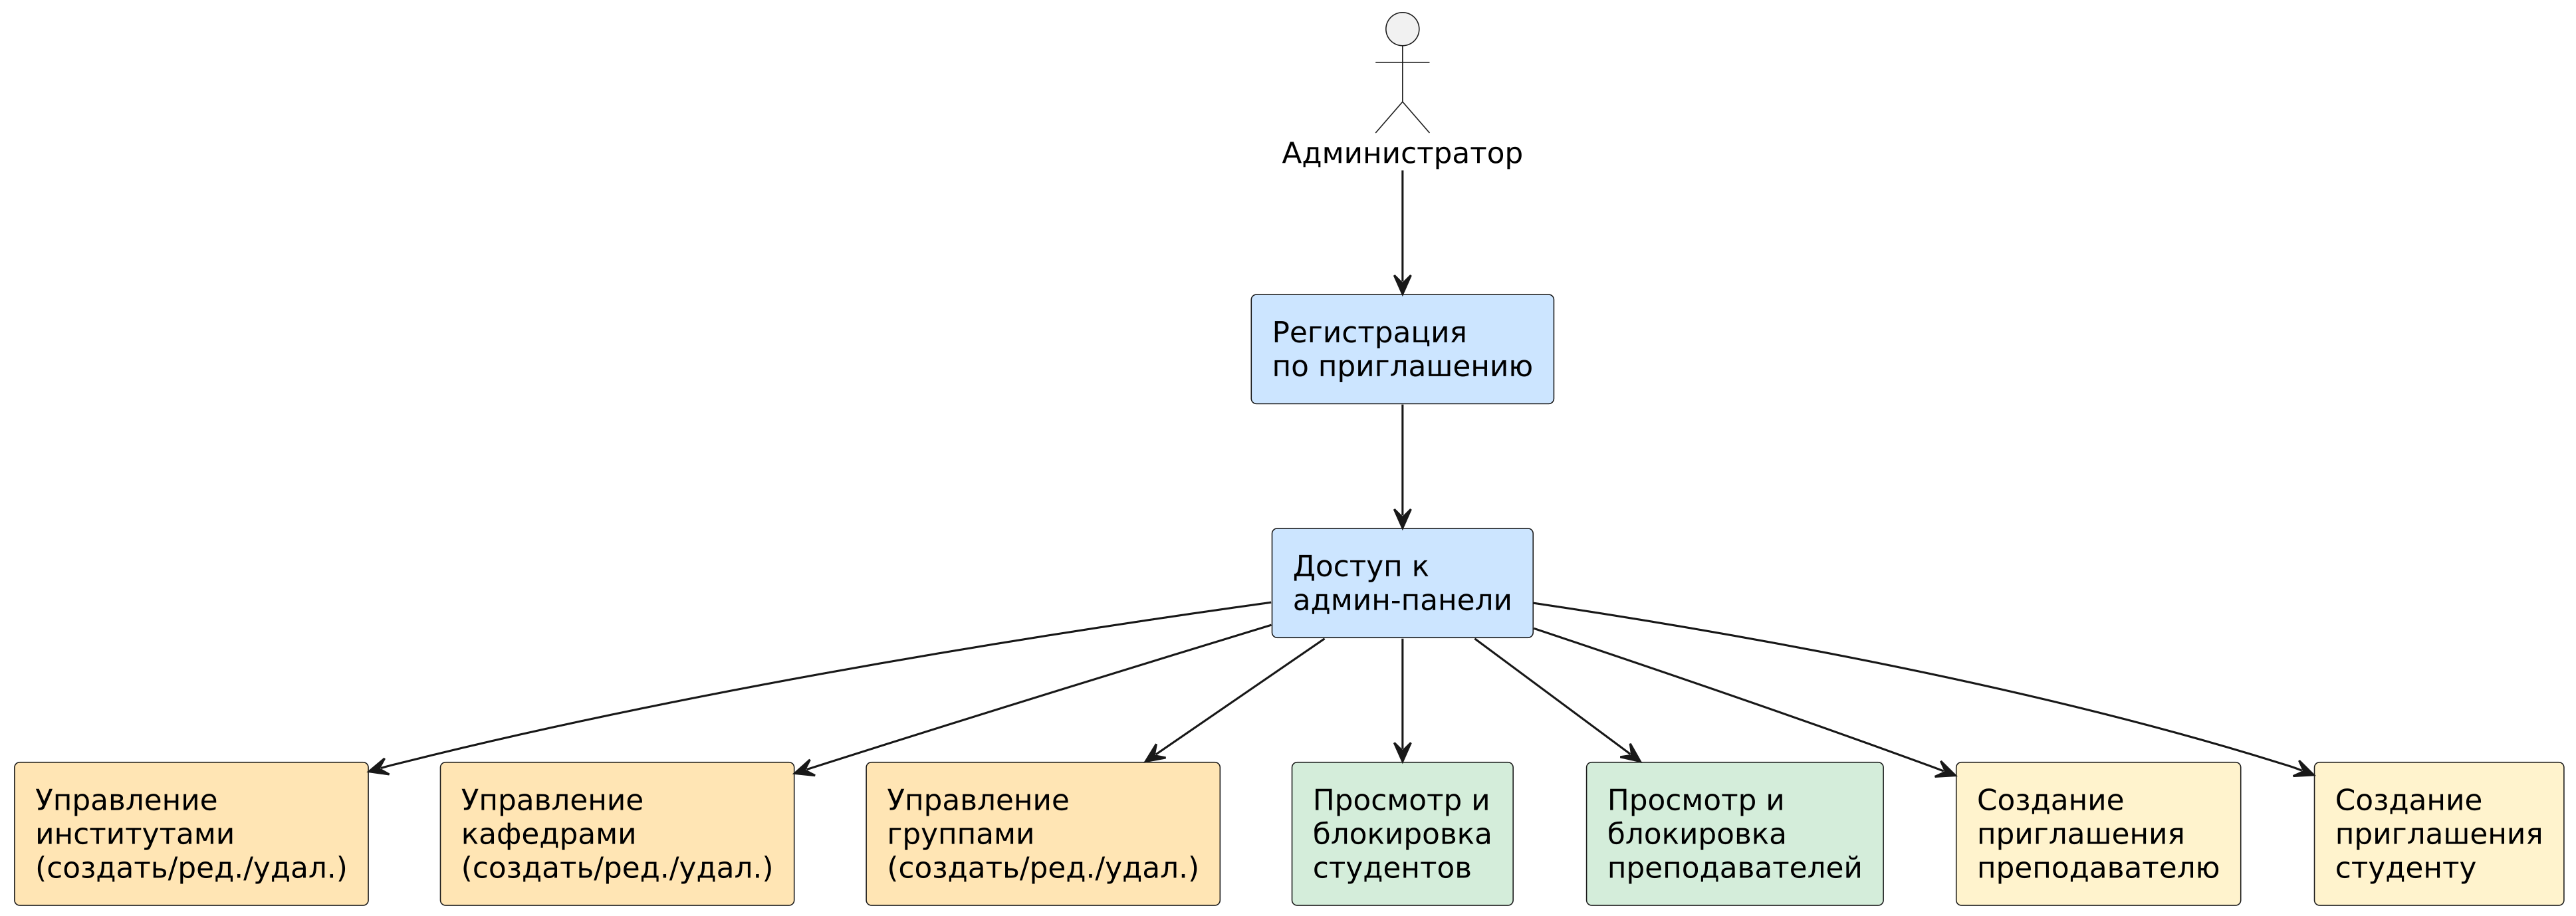
\includegraphics[width=\linewidth]{static/AdminFlowchart.png}
    \vspace{0.5em}
    {\small Диаграмма действий администратора}
\end{frame}

\begin{frame}{Взаимодействие преподавателя с web-приложением}
    \centering
    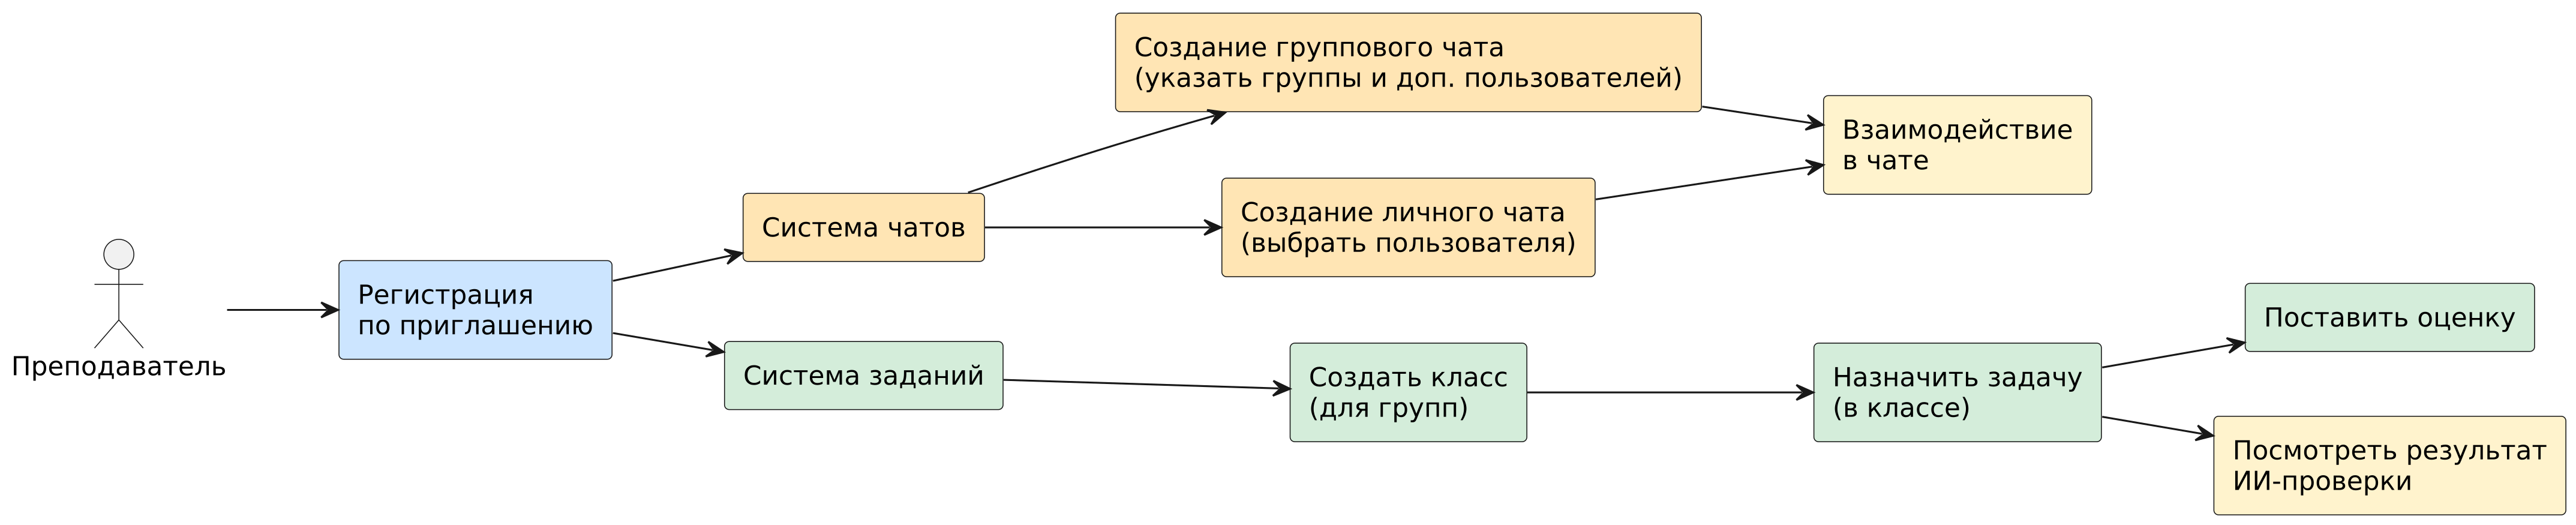
\includegraphics[width=\linewidth]{static/TeacherFlowchart.png}
    \vspace{0.5em}
    {\small Диаграмма действий преподавателя}
\end{frame}

\begin{frame}{Взаимодействие студента с web-приложением}
    \centering
    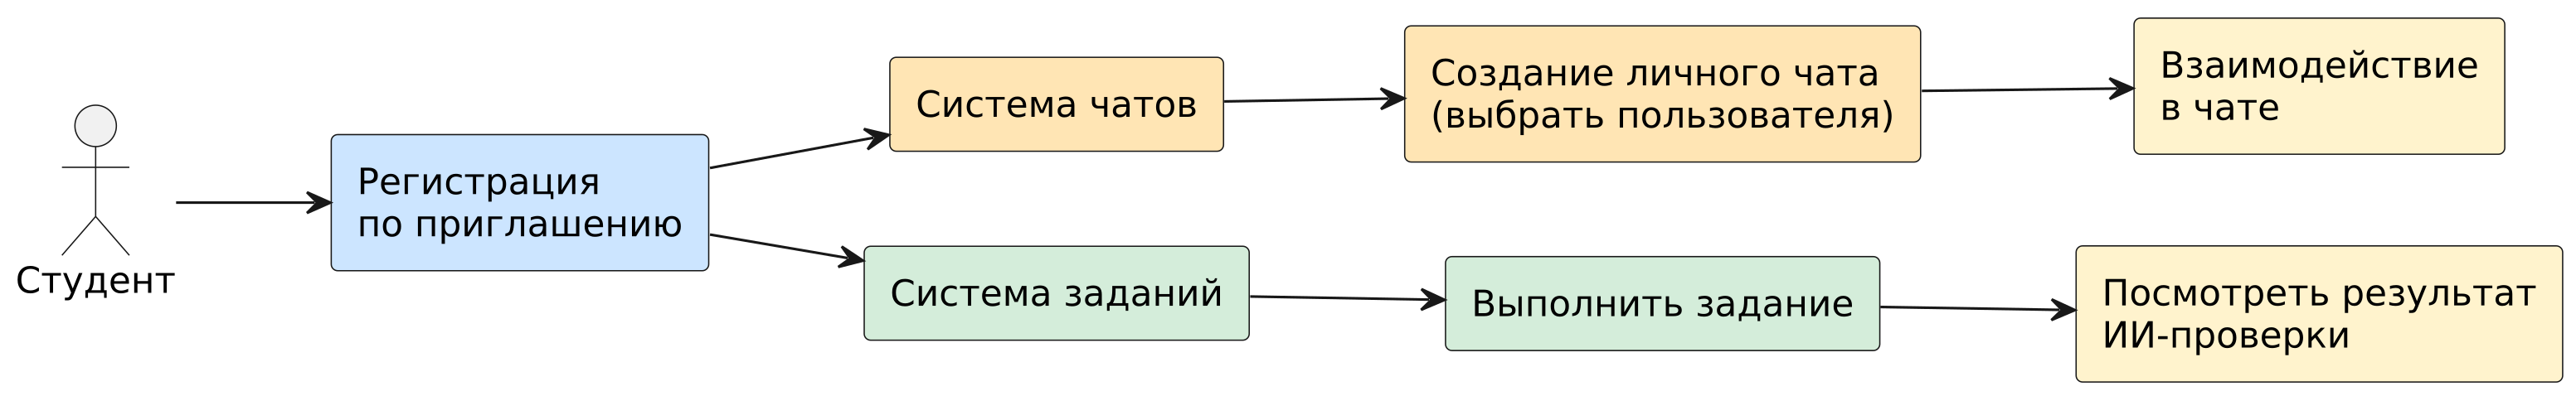
\includegraphics[width=\linewidth]{static/StudentFlowchart.png}
    \vspace{0.5em}
    {\small Диаграмма действий студента}
\end{frame}


%\begin{frame}{Создание приглашения пользователей}
%\vspace{0.5em}
%
%\centering
%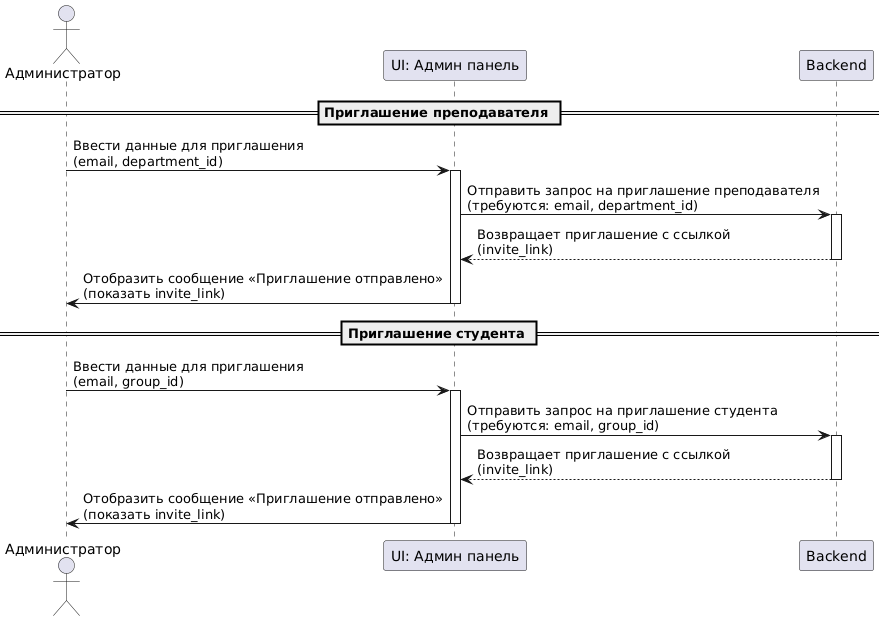
\includegraphics[width=0.7\linewidth]{static/Admin.png} \\
%\small Диаграмма приглашения пользователей 
%\end{frame}
%
%
%\begin{frame}{Регистрация}
%\centering
%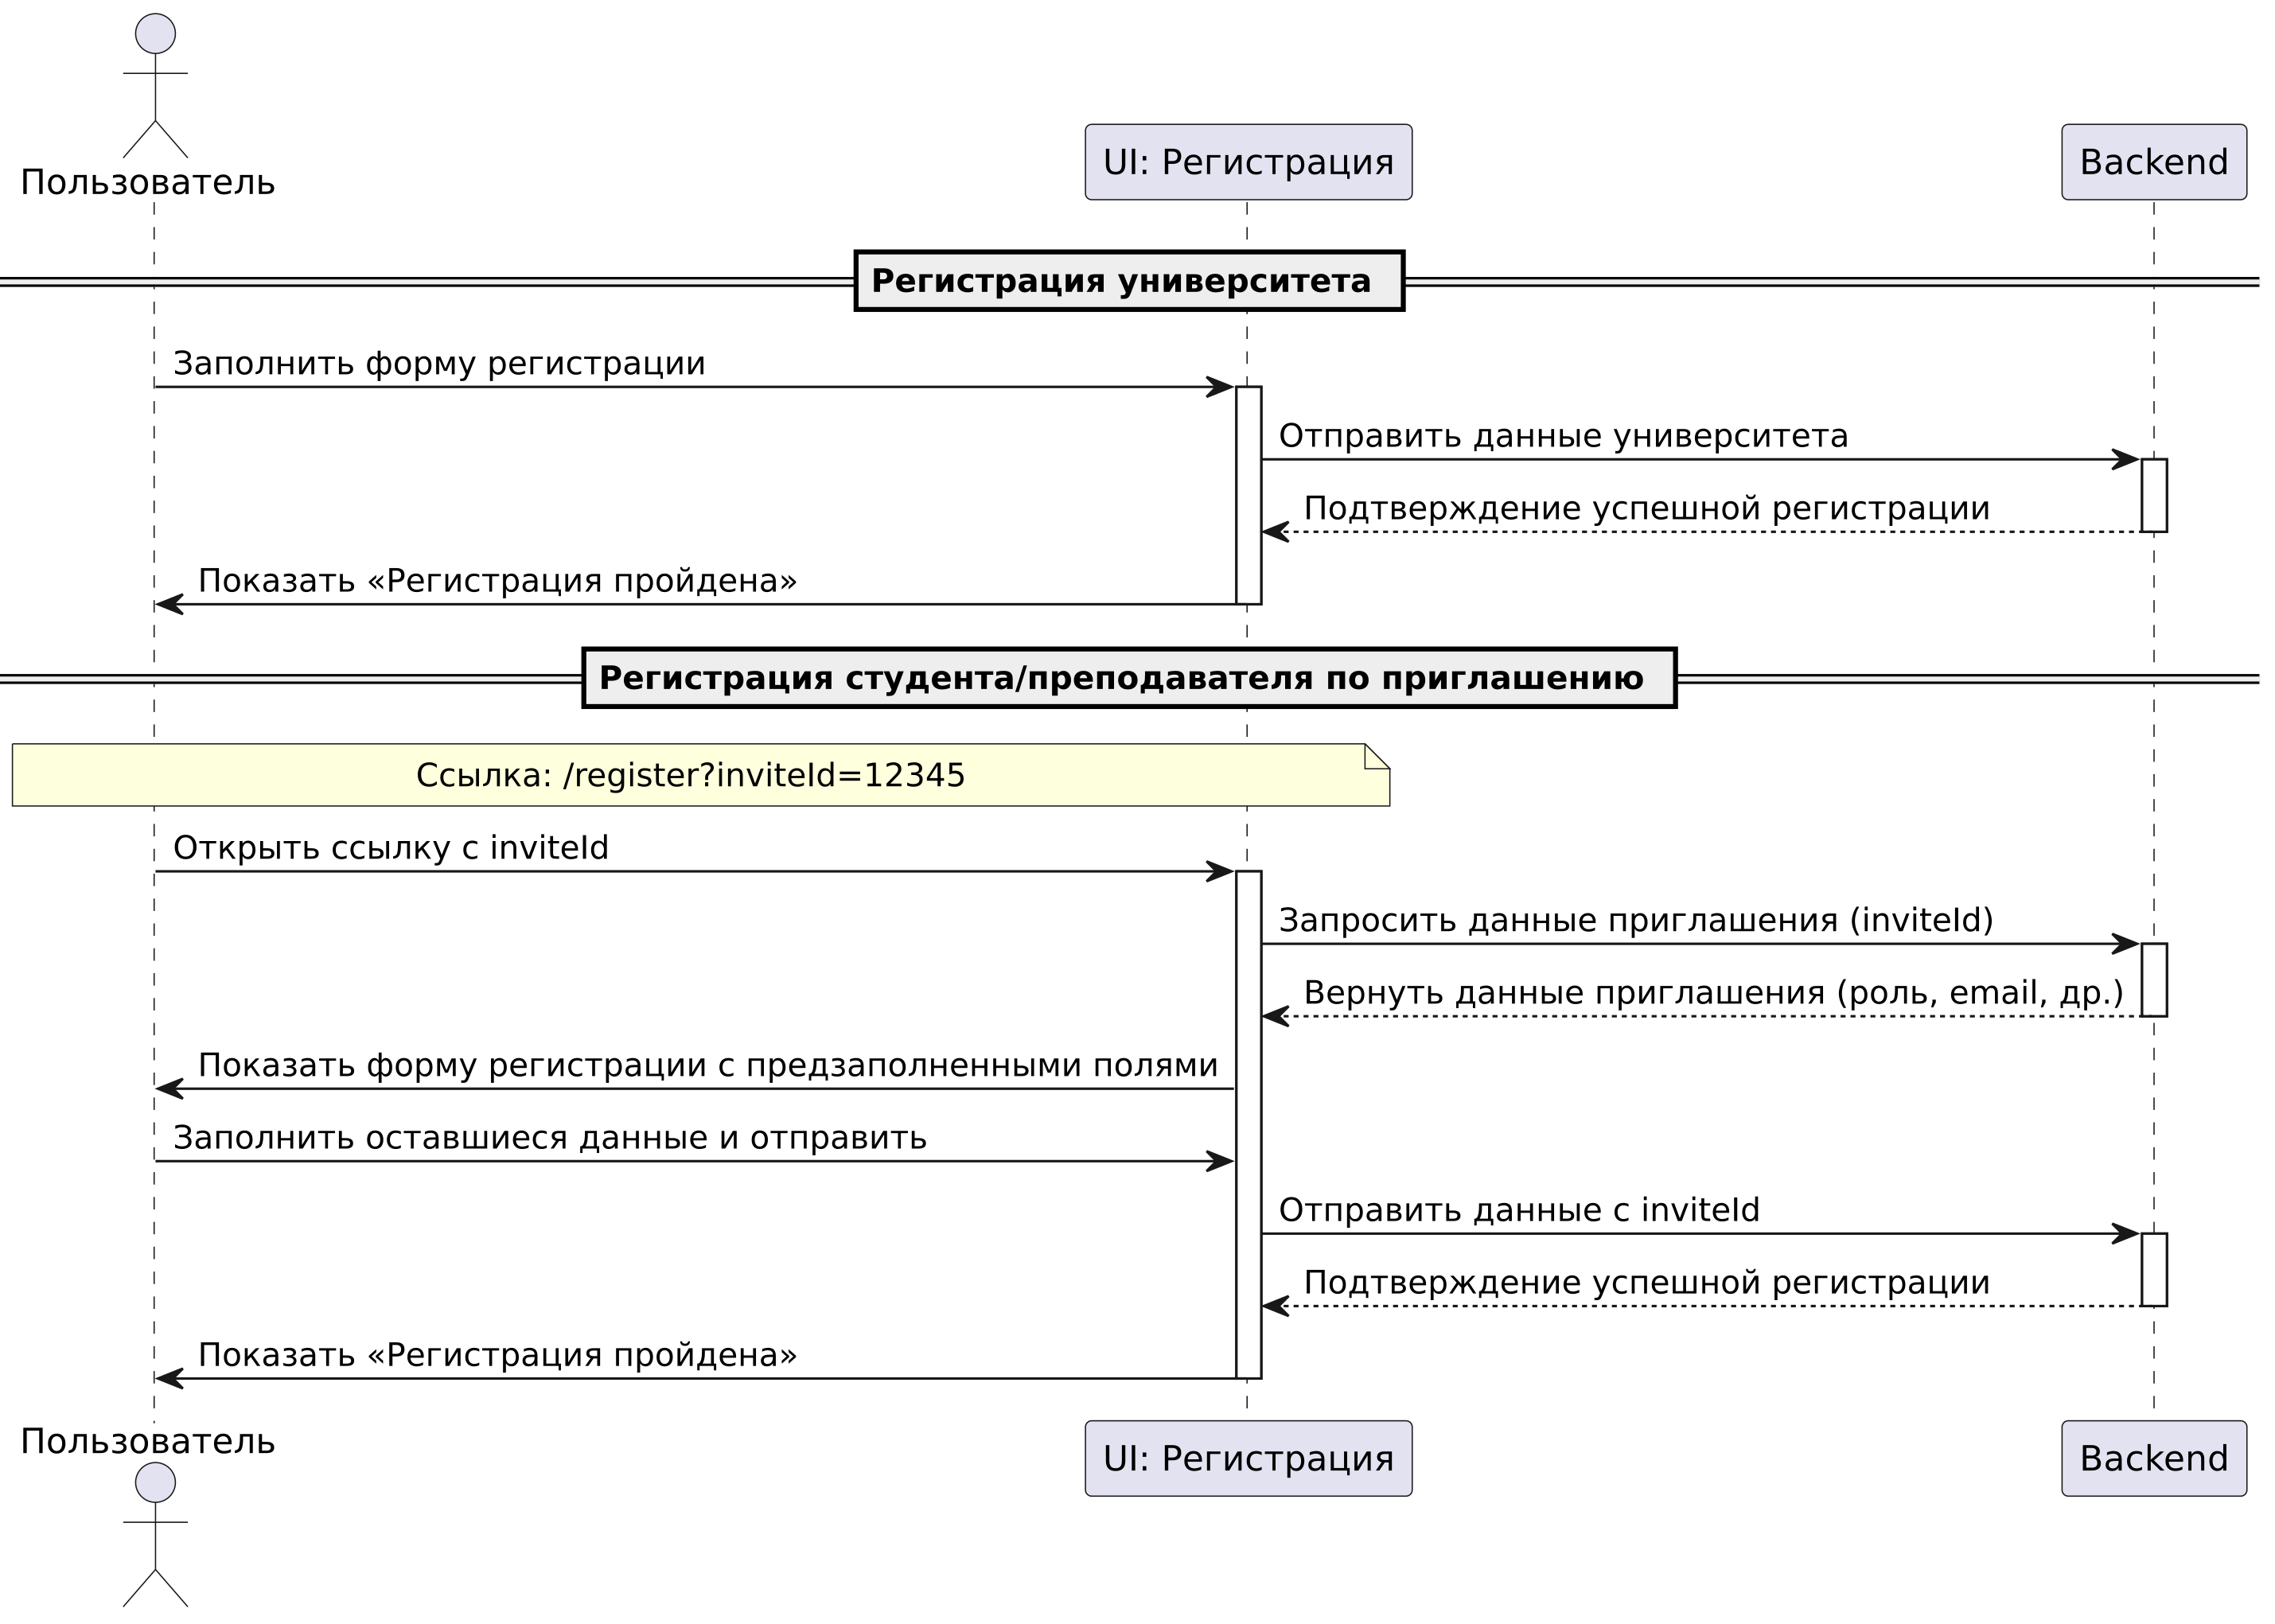
\includegraphics[width=0.7\linewidth]{static/RegistrationDiagrams.png} \\
%\small Диаграмма регистрации пользователя
%\end{frame}



%\begin{frame}{Создание класса}
%\vspace{0.5em}
%
%\begin{columns}
%    \begin{column}{0.5\textwidth}
%        \centering
%        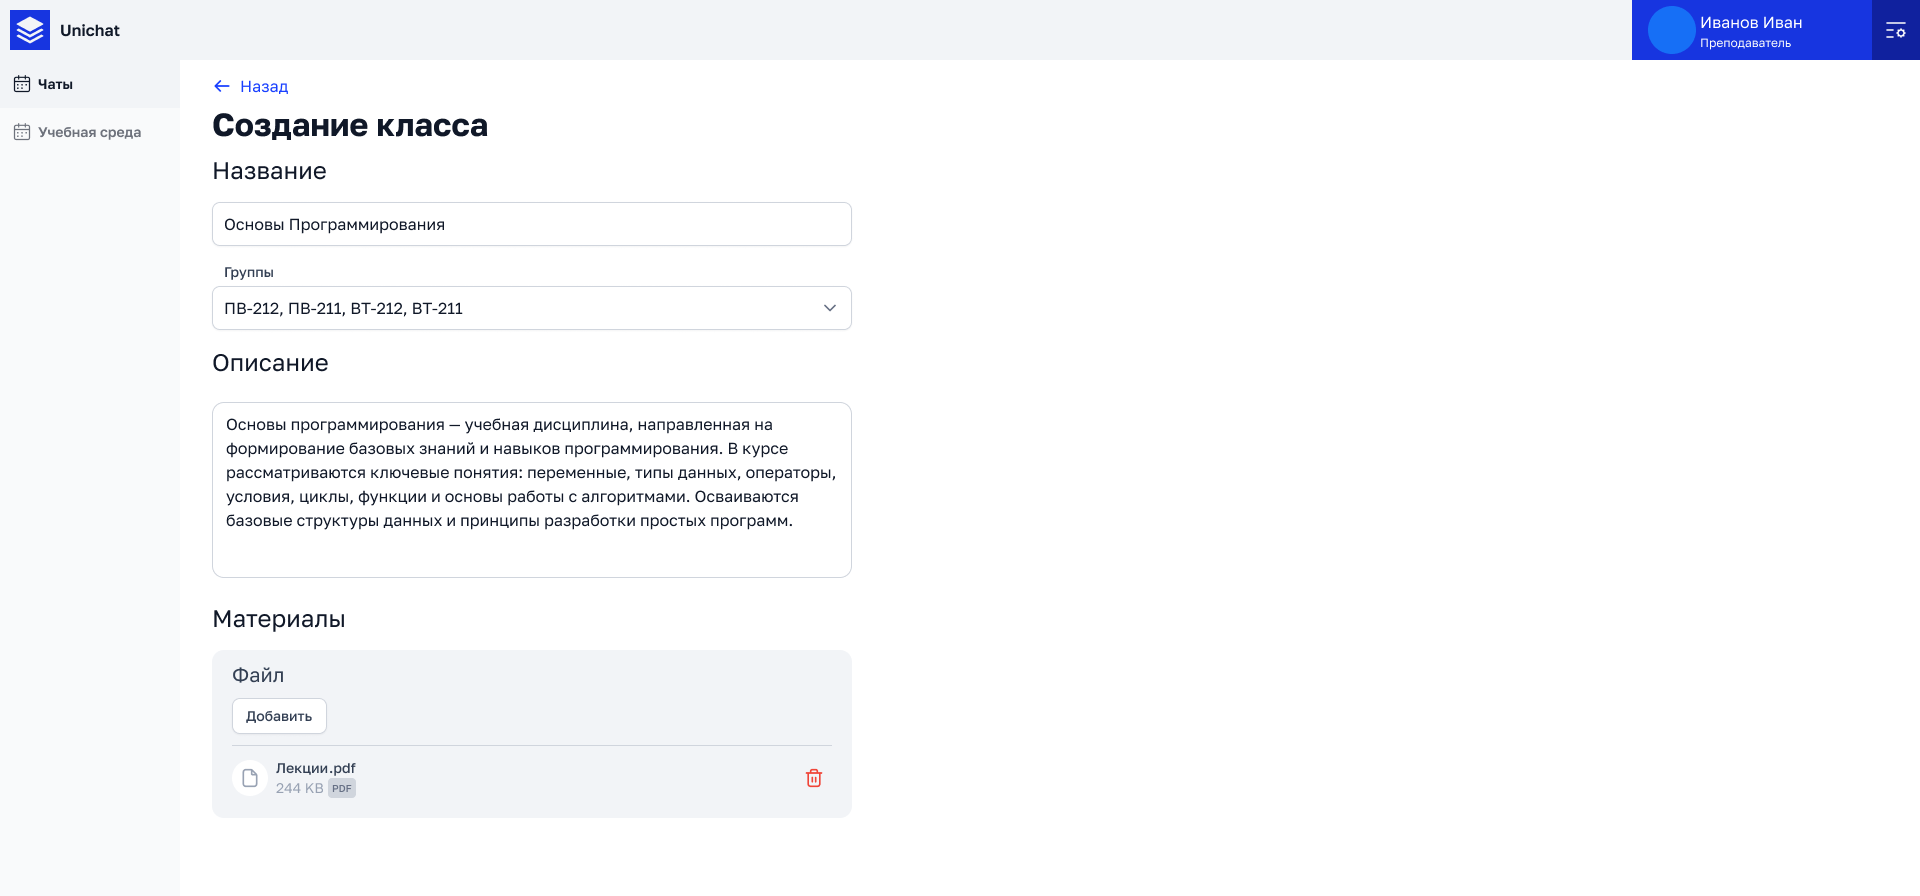
\includegraphics[width=0.95\linewidth]{static/ClassRoomCreate.png} \\
%        \small Интерфейс создания класса
%    \end{column}
%    \begin{column}{0.5\textwidth}
%        \centering
%        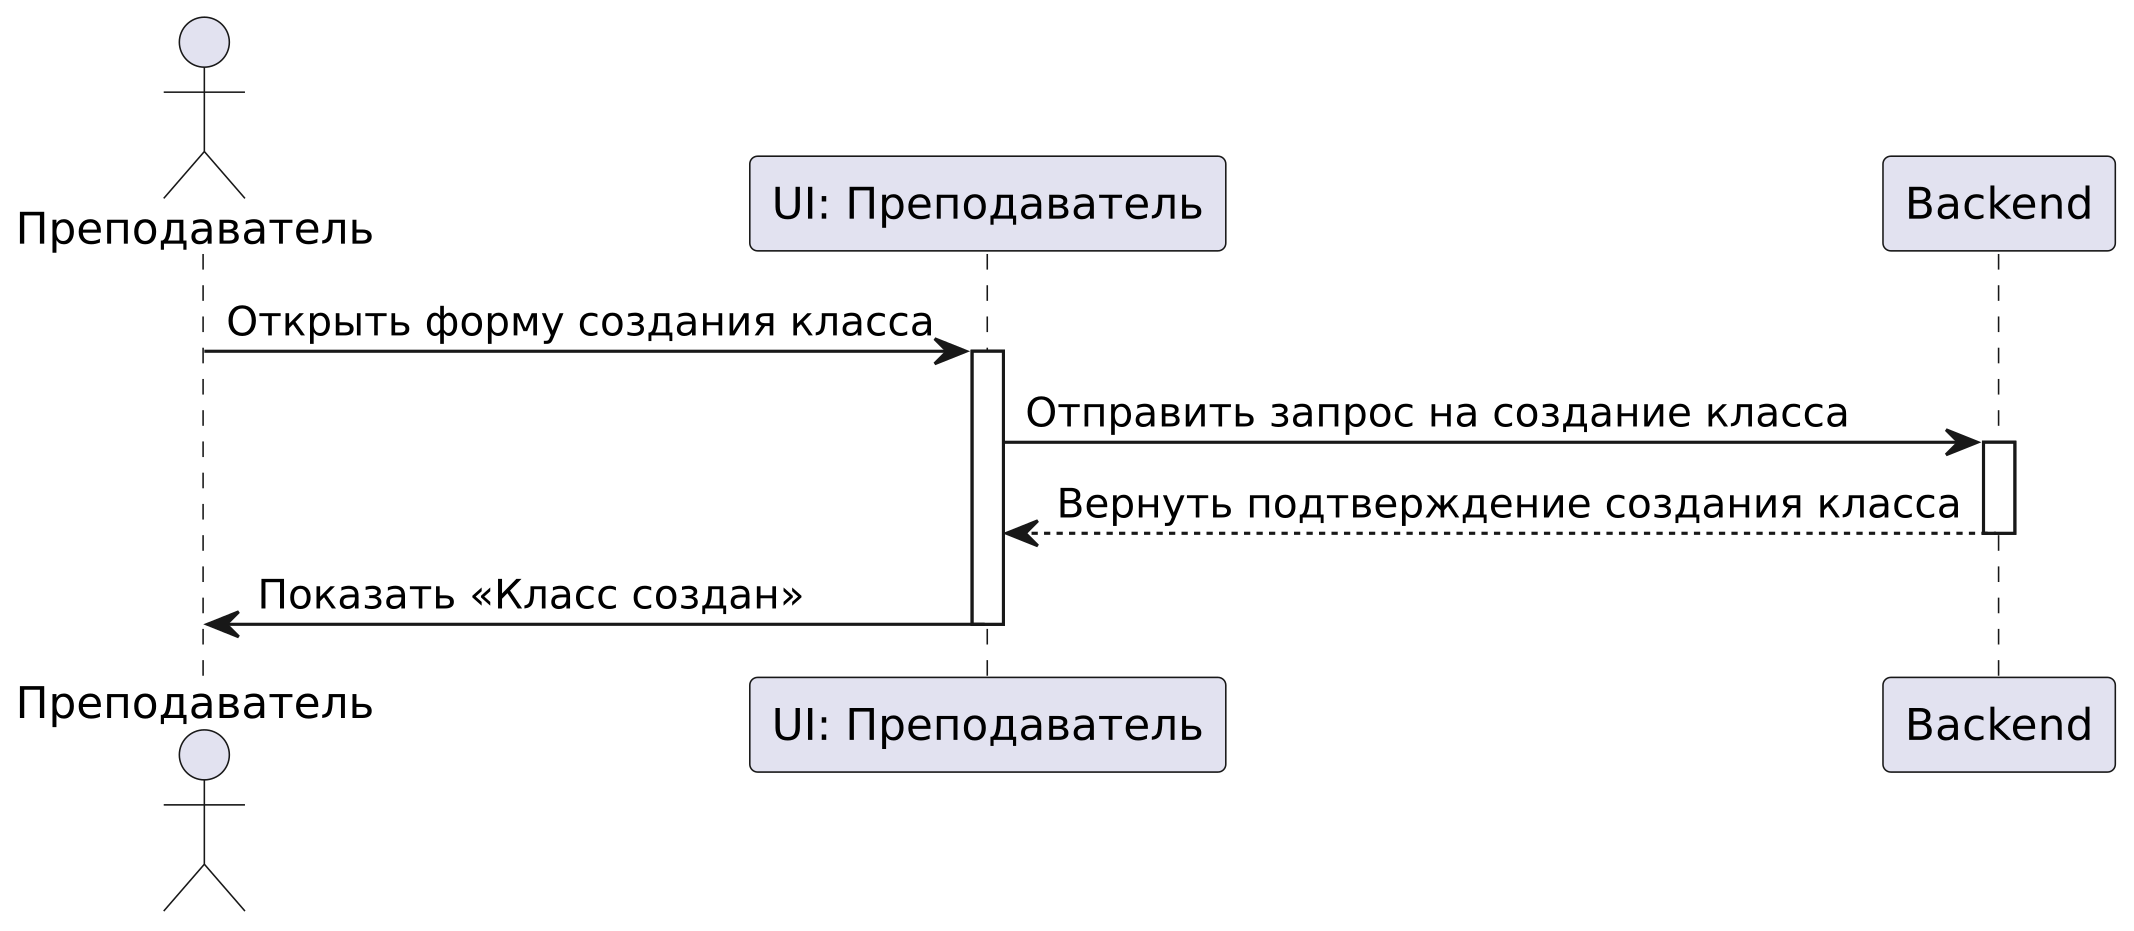
\includegraphics[width=0.95\linewidth]{static/ClassRoomCreateDiagram.png} \\
%        \small Диаграмма создания класса
%    \end{column}
%\end{columns}
%\end{frame}

\begin{frame}{Создание задачи}
\vspace{0.5em}

\begin{columns}
    \begin{column}{0.5\textwidth}
        \centering
        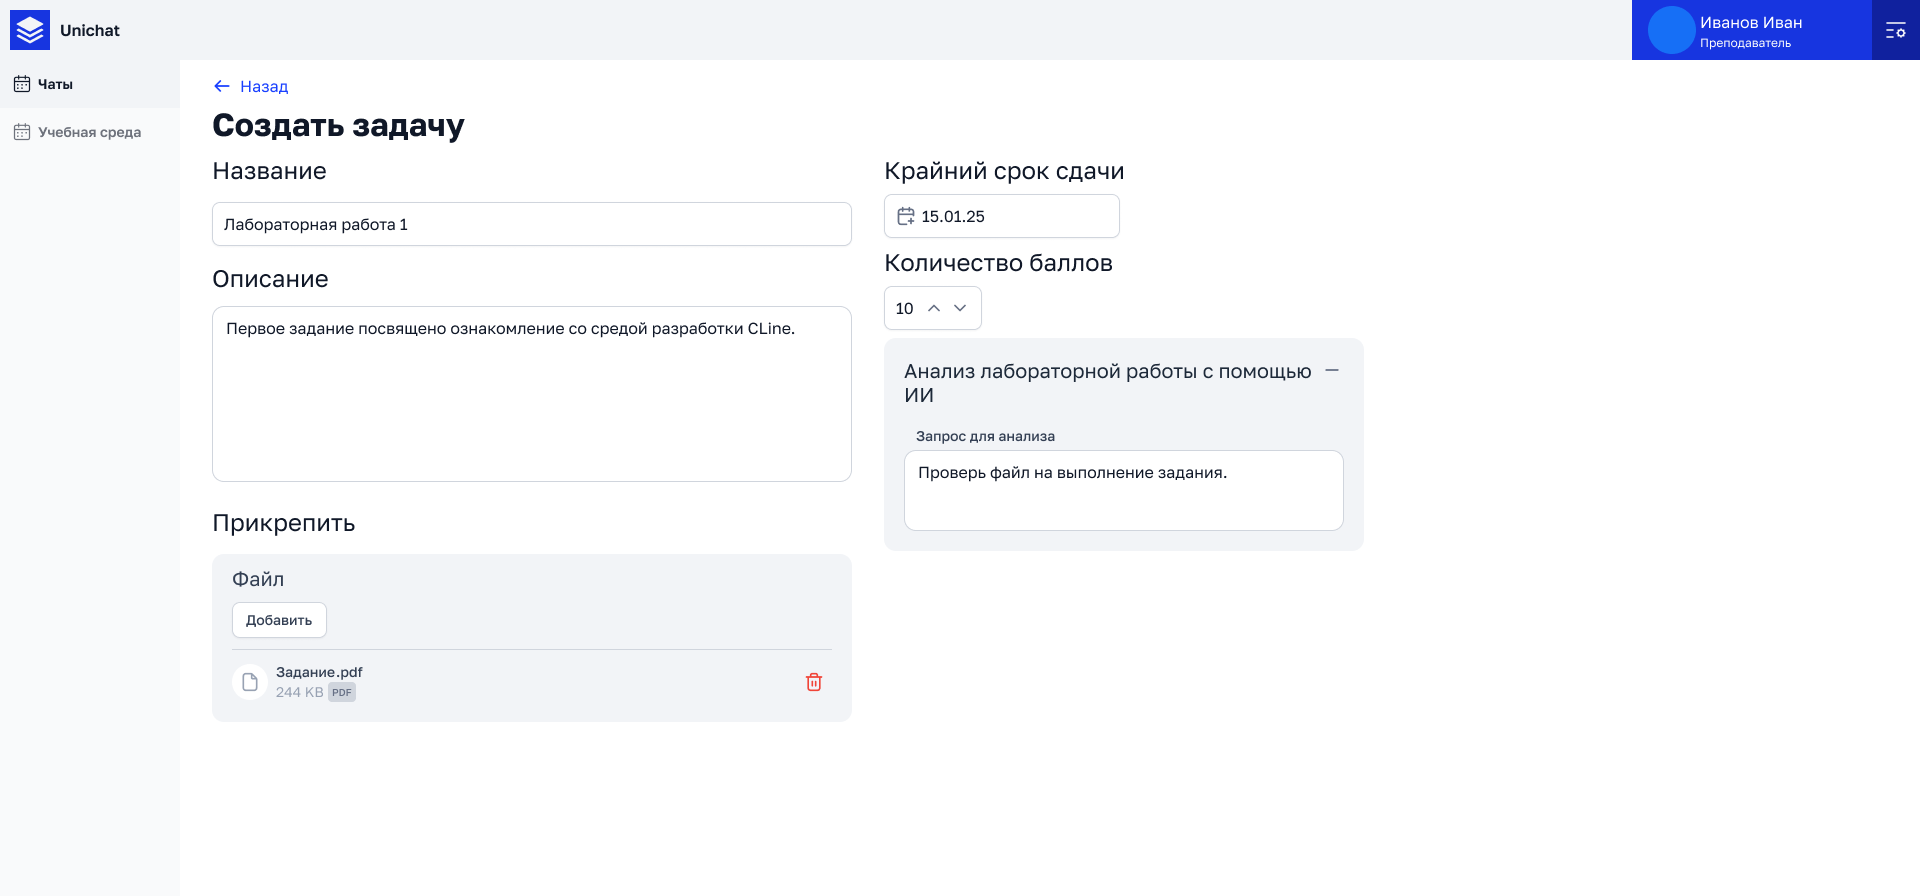
\includegraphics[width=\linewidth]{static/TaskCreate.png} \\
        \small Интерфейс создания задачи
    \end{column}
    \begin{column}{0.5\textwidth}
        \centering
        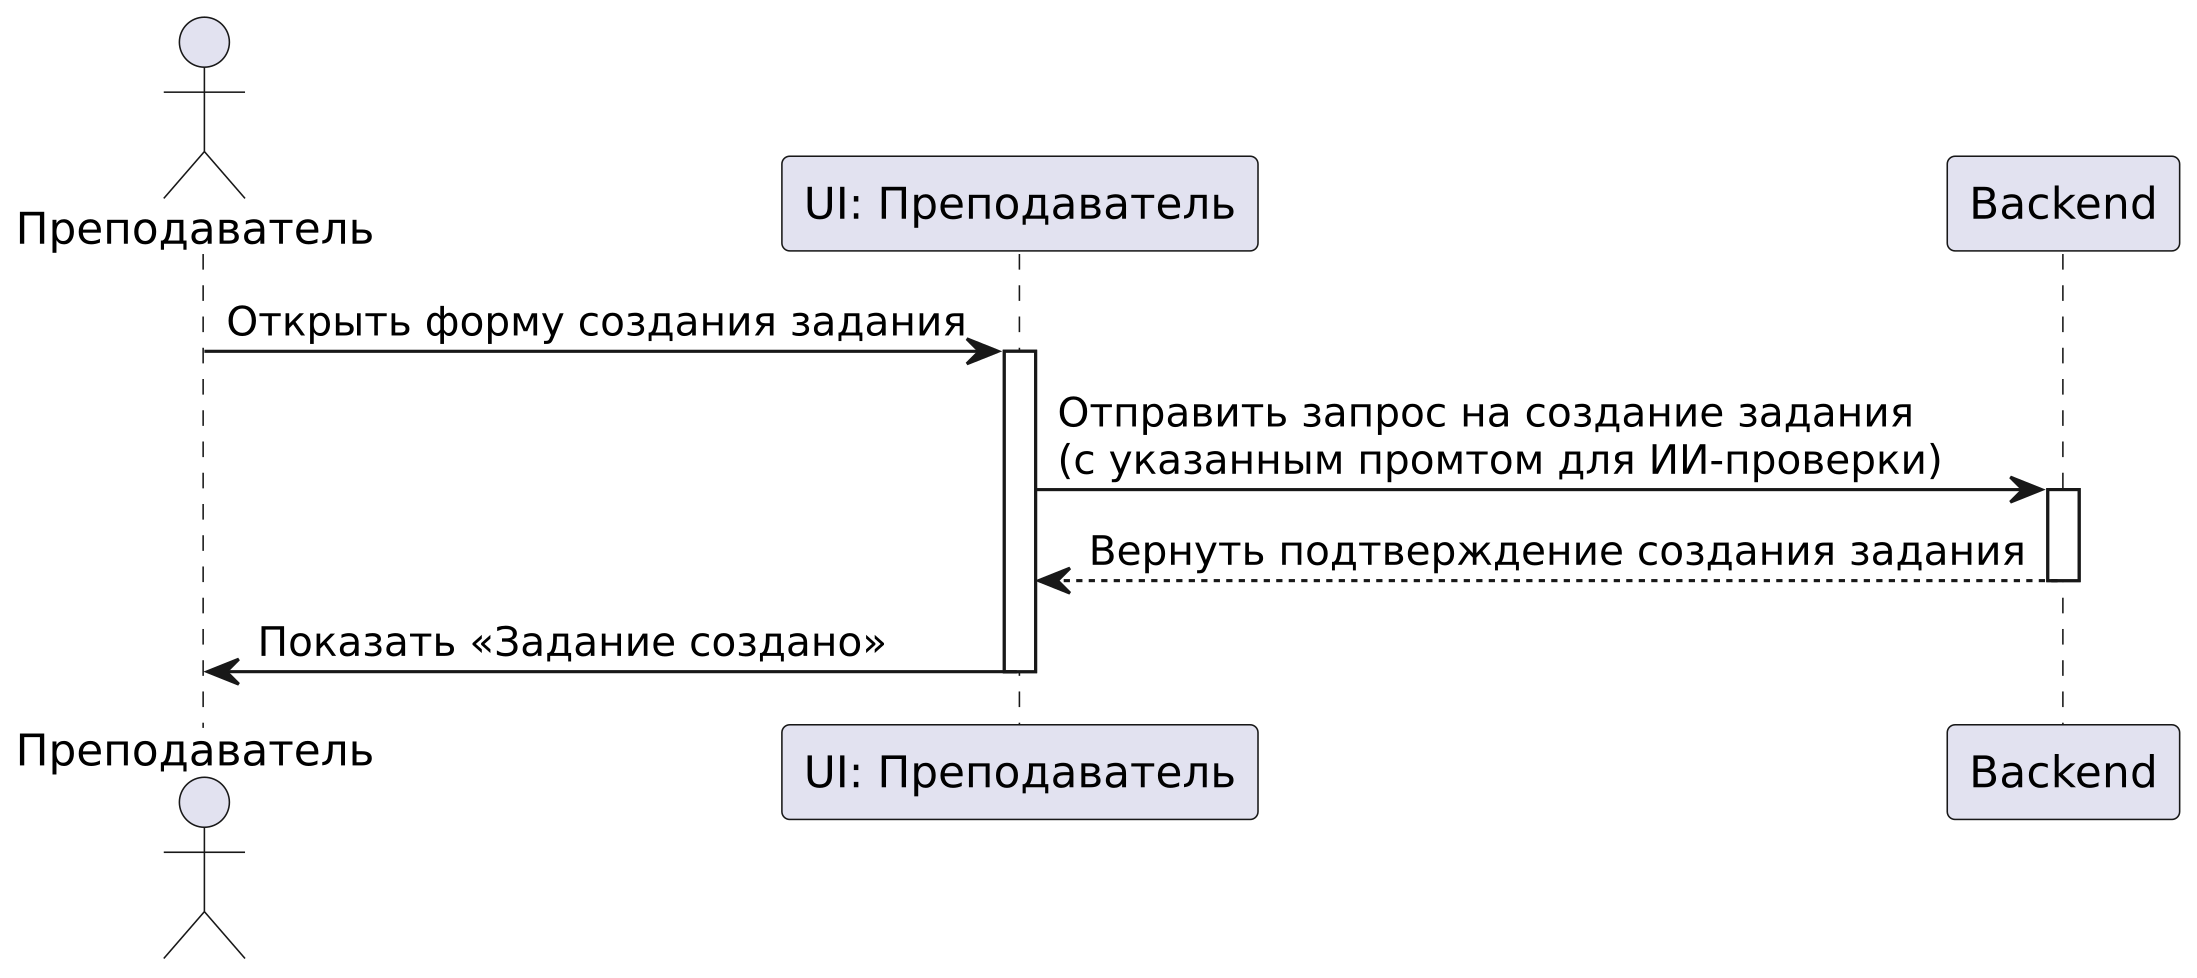
\includegraphics[width=\linewidth]{static/TaskCreateDiagram.png} \\
        \small Диаграмма создания задачи
    \end{column}
\end{columns}
\end{frame}


\begin{frame}{Отправка задания на проверку}
\vspace{0.5em}

\centering
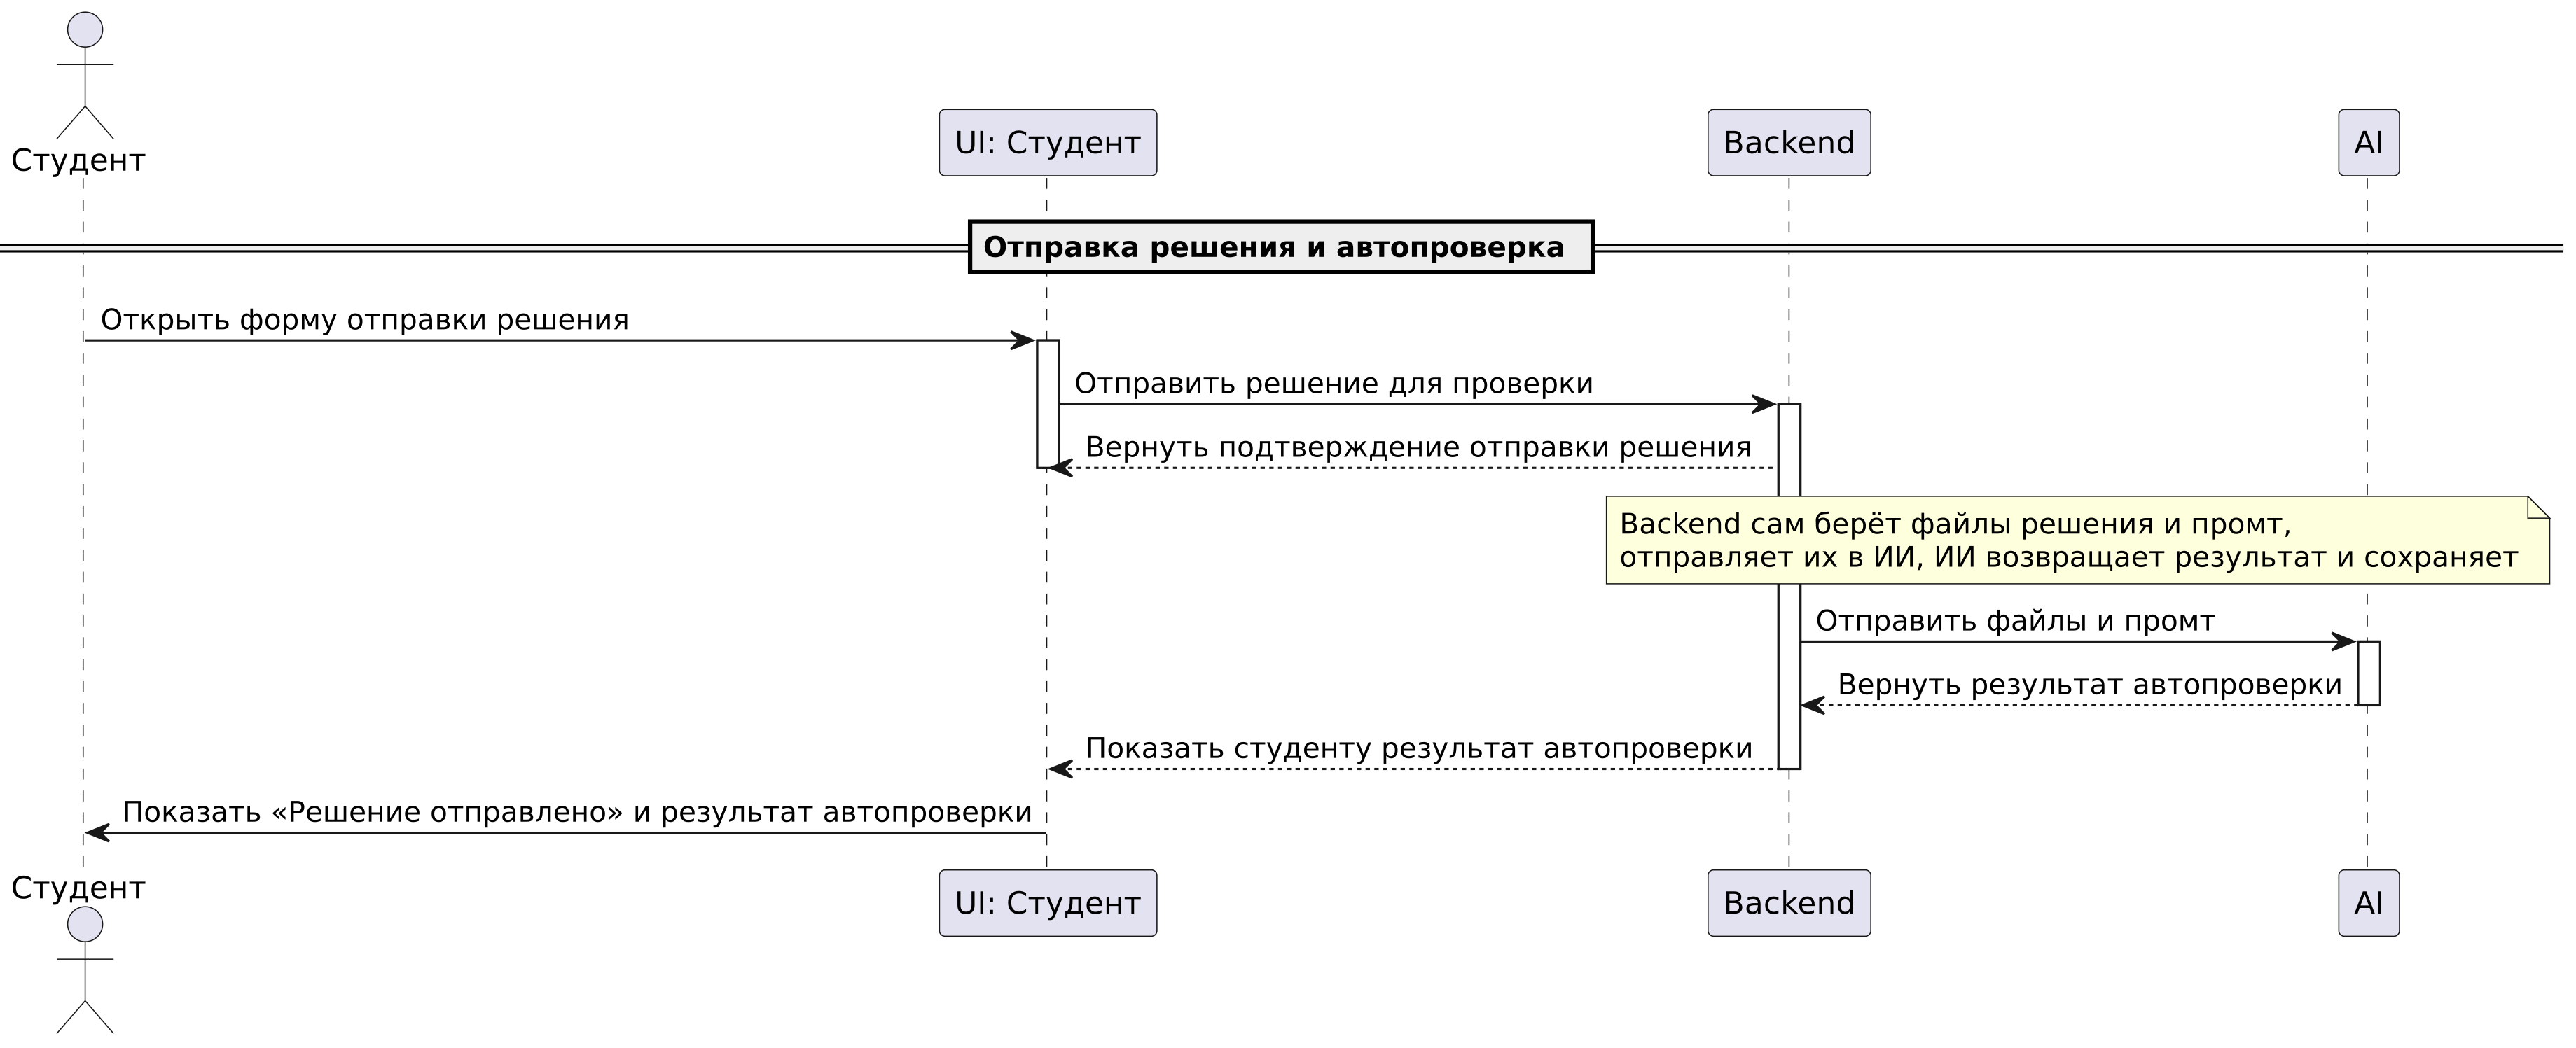
\includegraphics[width=0.75\linewidth]{static/TaskSendStudentDiagram.png} \\
\small Диаграмма взаимодействия при просмотре задания конкретного студента
\end{frame}

\begin{frame}{Интерфейс задания определённого студента}
\vspace{0.5em}

\begin{columns}
    \begin{column}{0.5\textwidth}
        \centering
        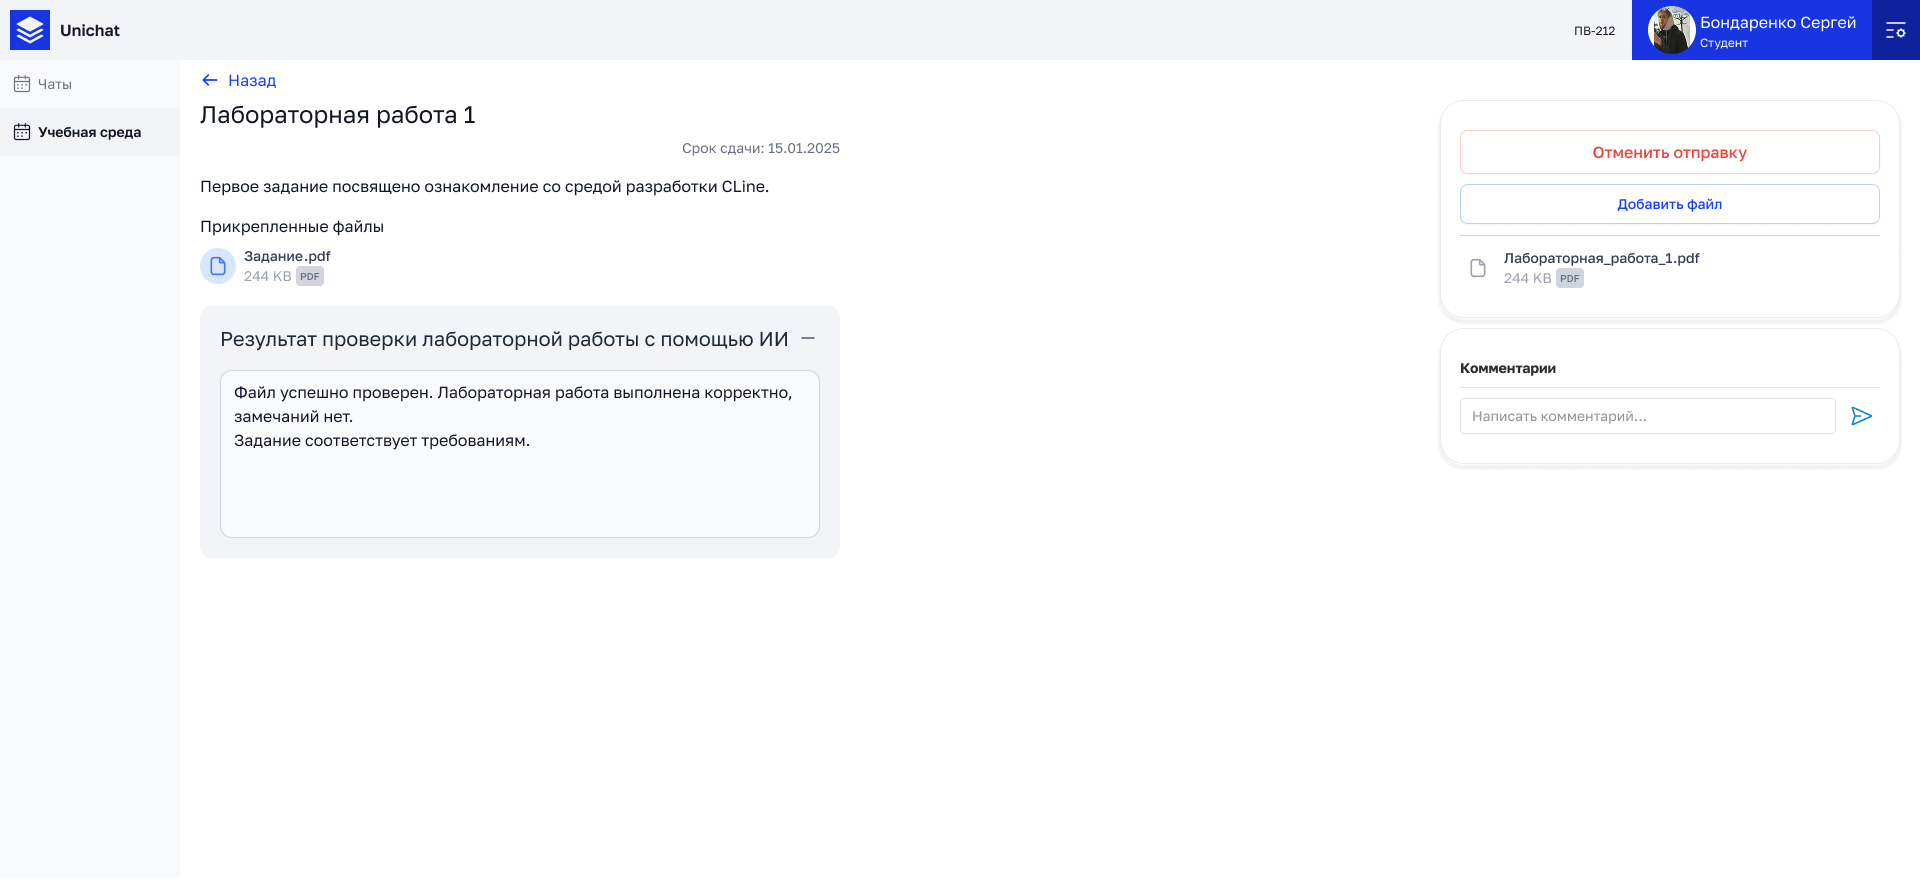
\includegraphics[width=0.95\linewidth]{static/TaskStudentSend.png} \\
        \small Интерфейс задания со стороны студента
    \end{column}
    \begin{column}{0.5\textwidth}
        \centering
        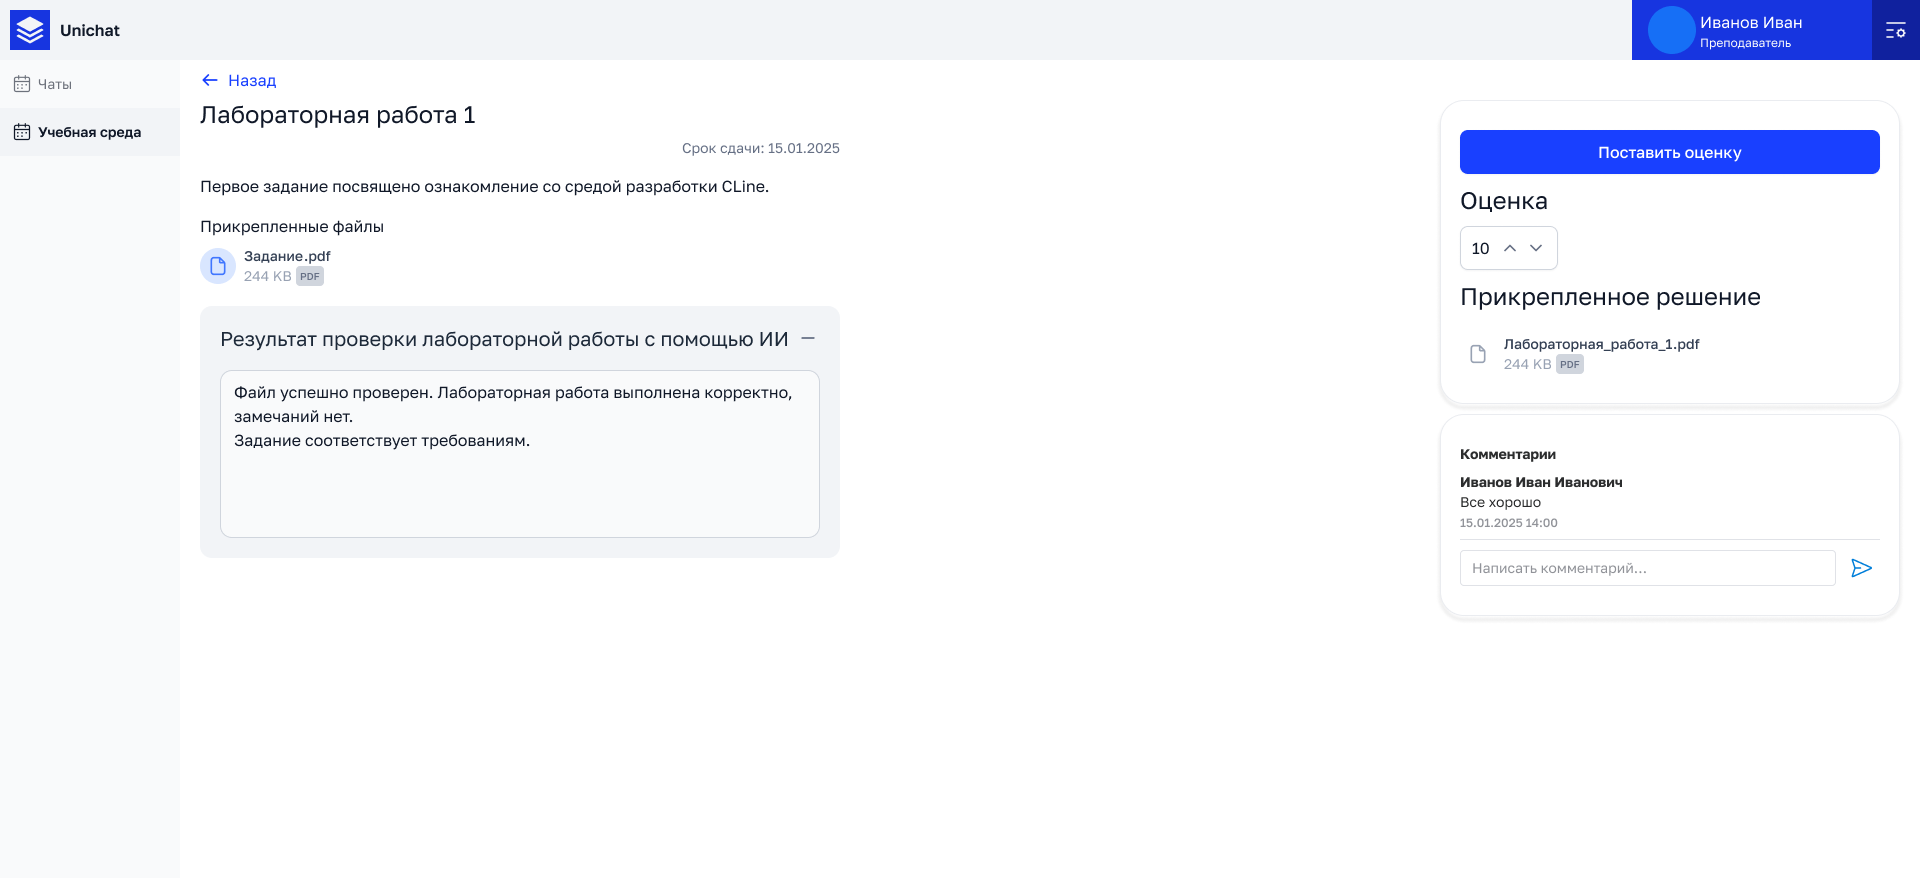
\includegraphics[width=0.95\linewidth]{static/TaskTeacherDetailByStudent.png} \\
        \small Просмотр задания преподавателем
    \end{column}
\end{columns}
\end{frame}

\begin{frame}{Диаграммы взаимодействия с чатами}
\vspace{0.5em}

\begin{columns}
    \begin{column}{0.5\textwidth}
        \centering
        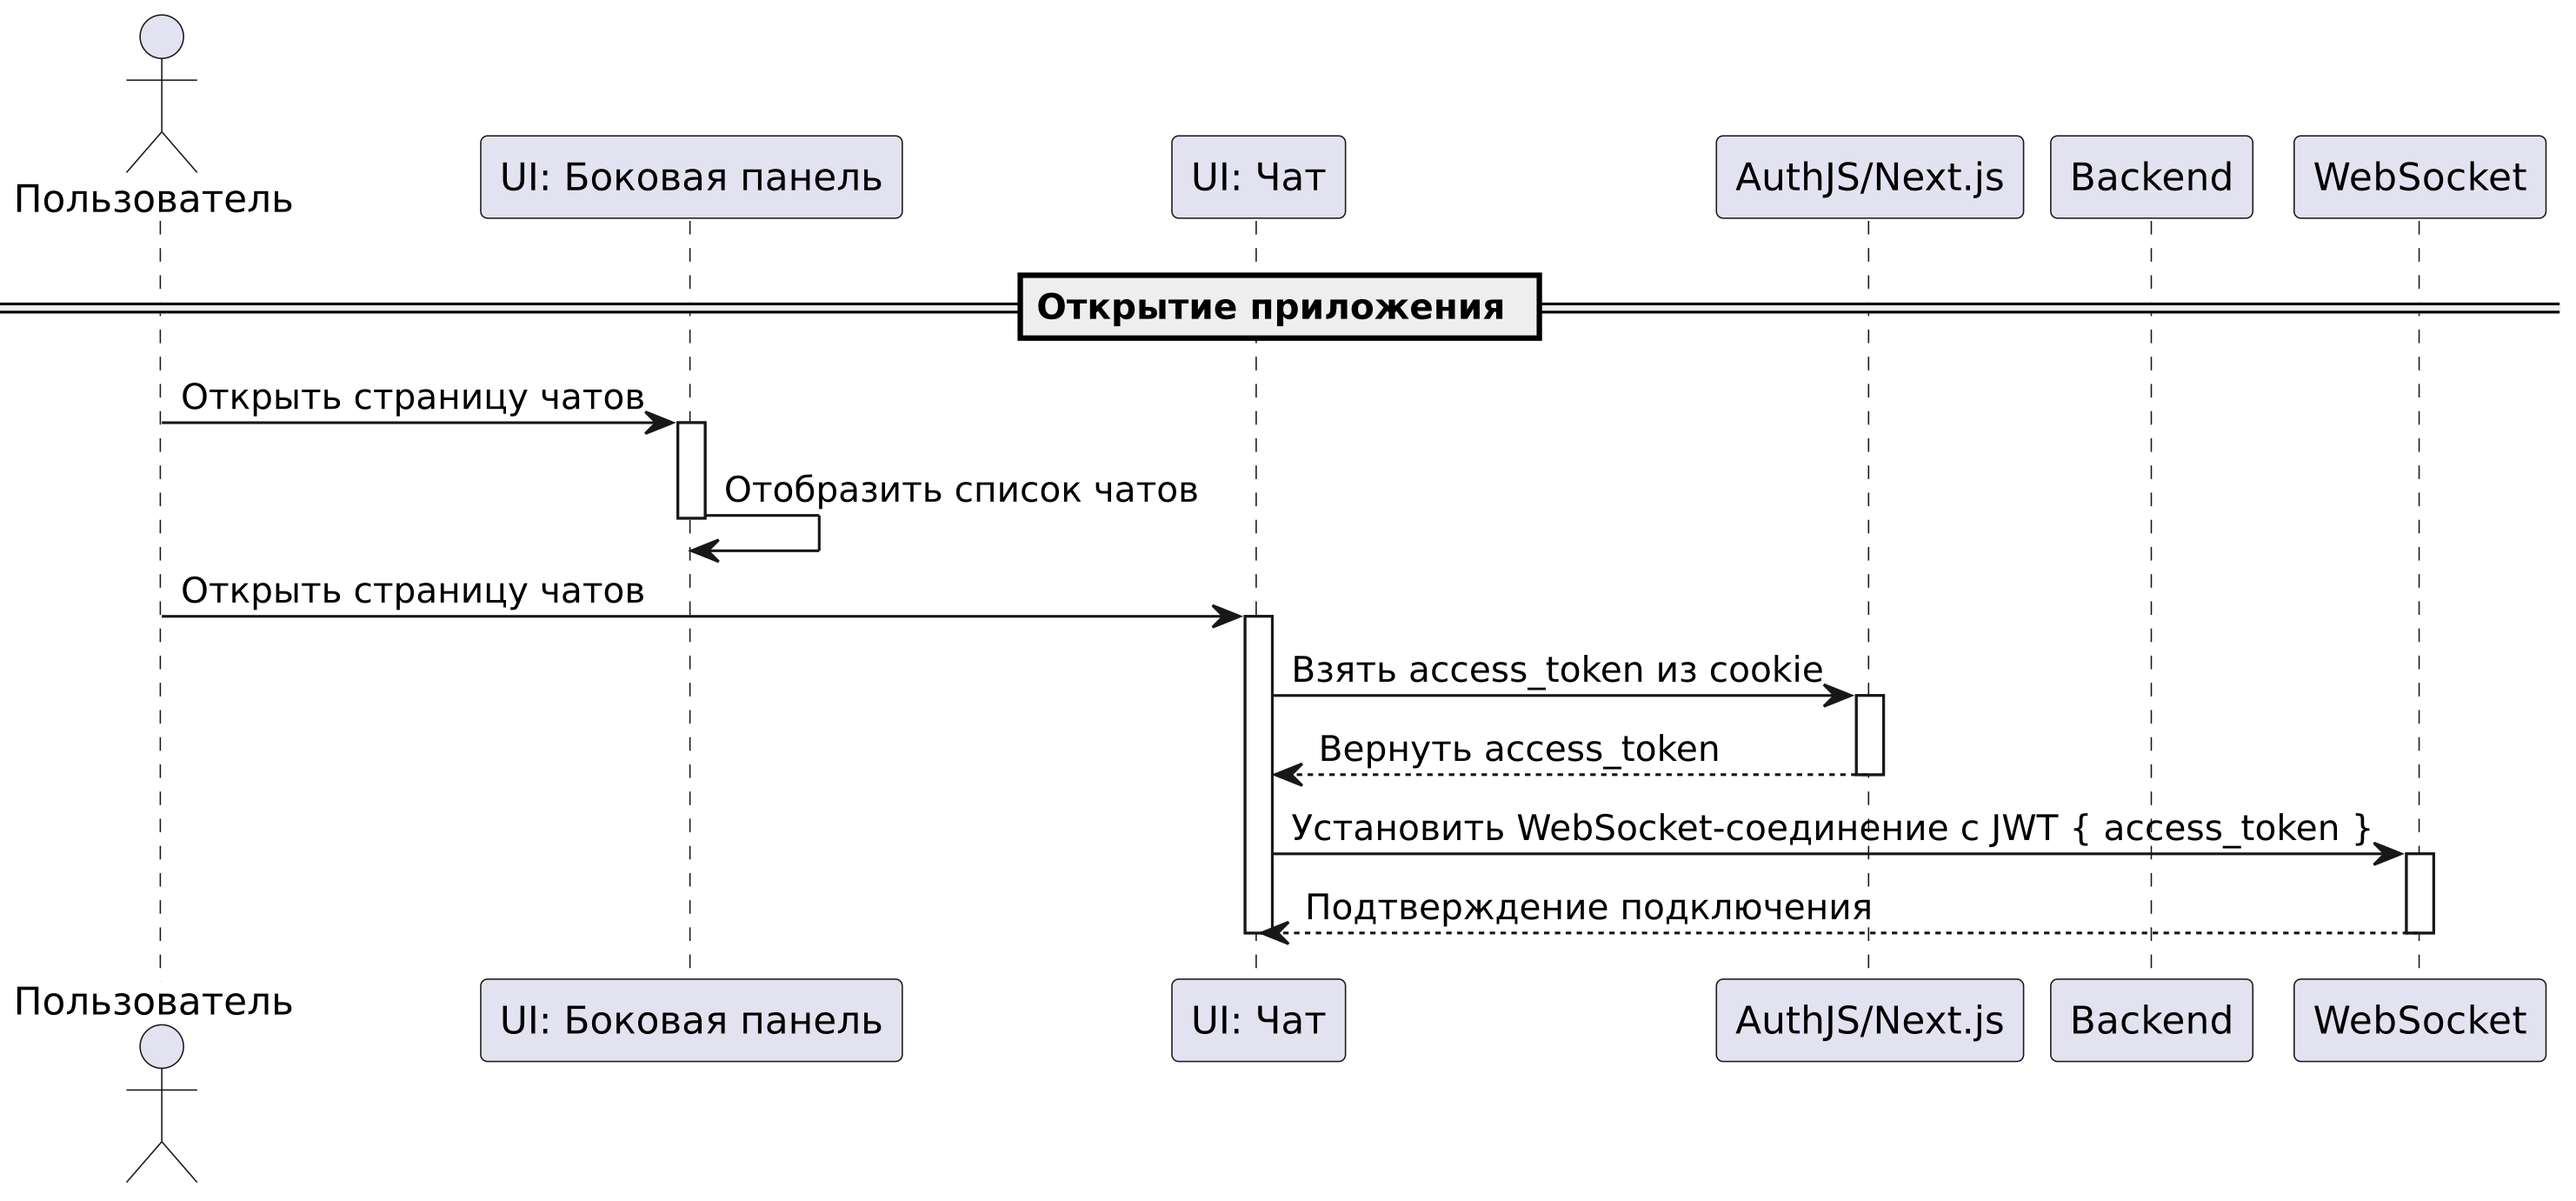
\includegraphics[width=0.95\linewidth]{static/ChatConnectDiagram.png} \\
        \small Подключение и инициализация чата
    \end{column}
    \begin{column}{0.5\textwidth}
        \centering
        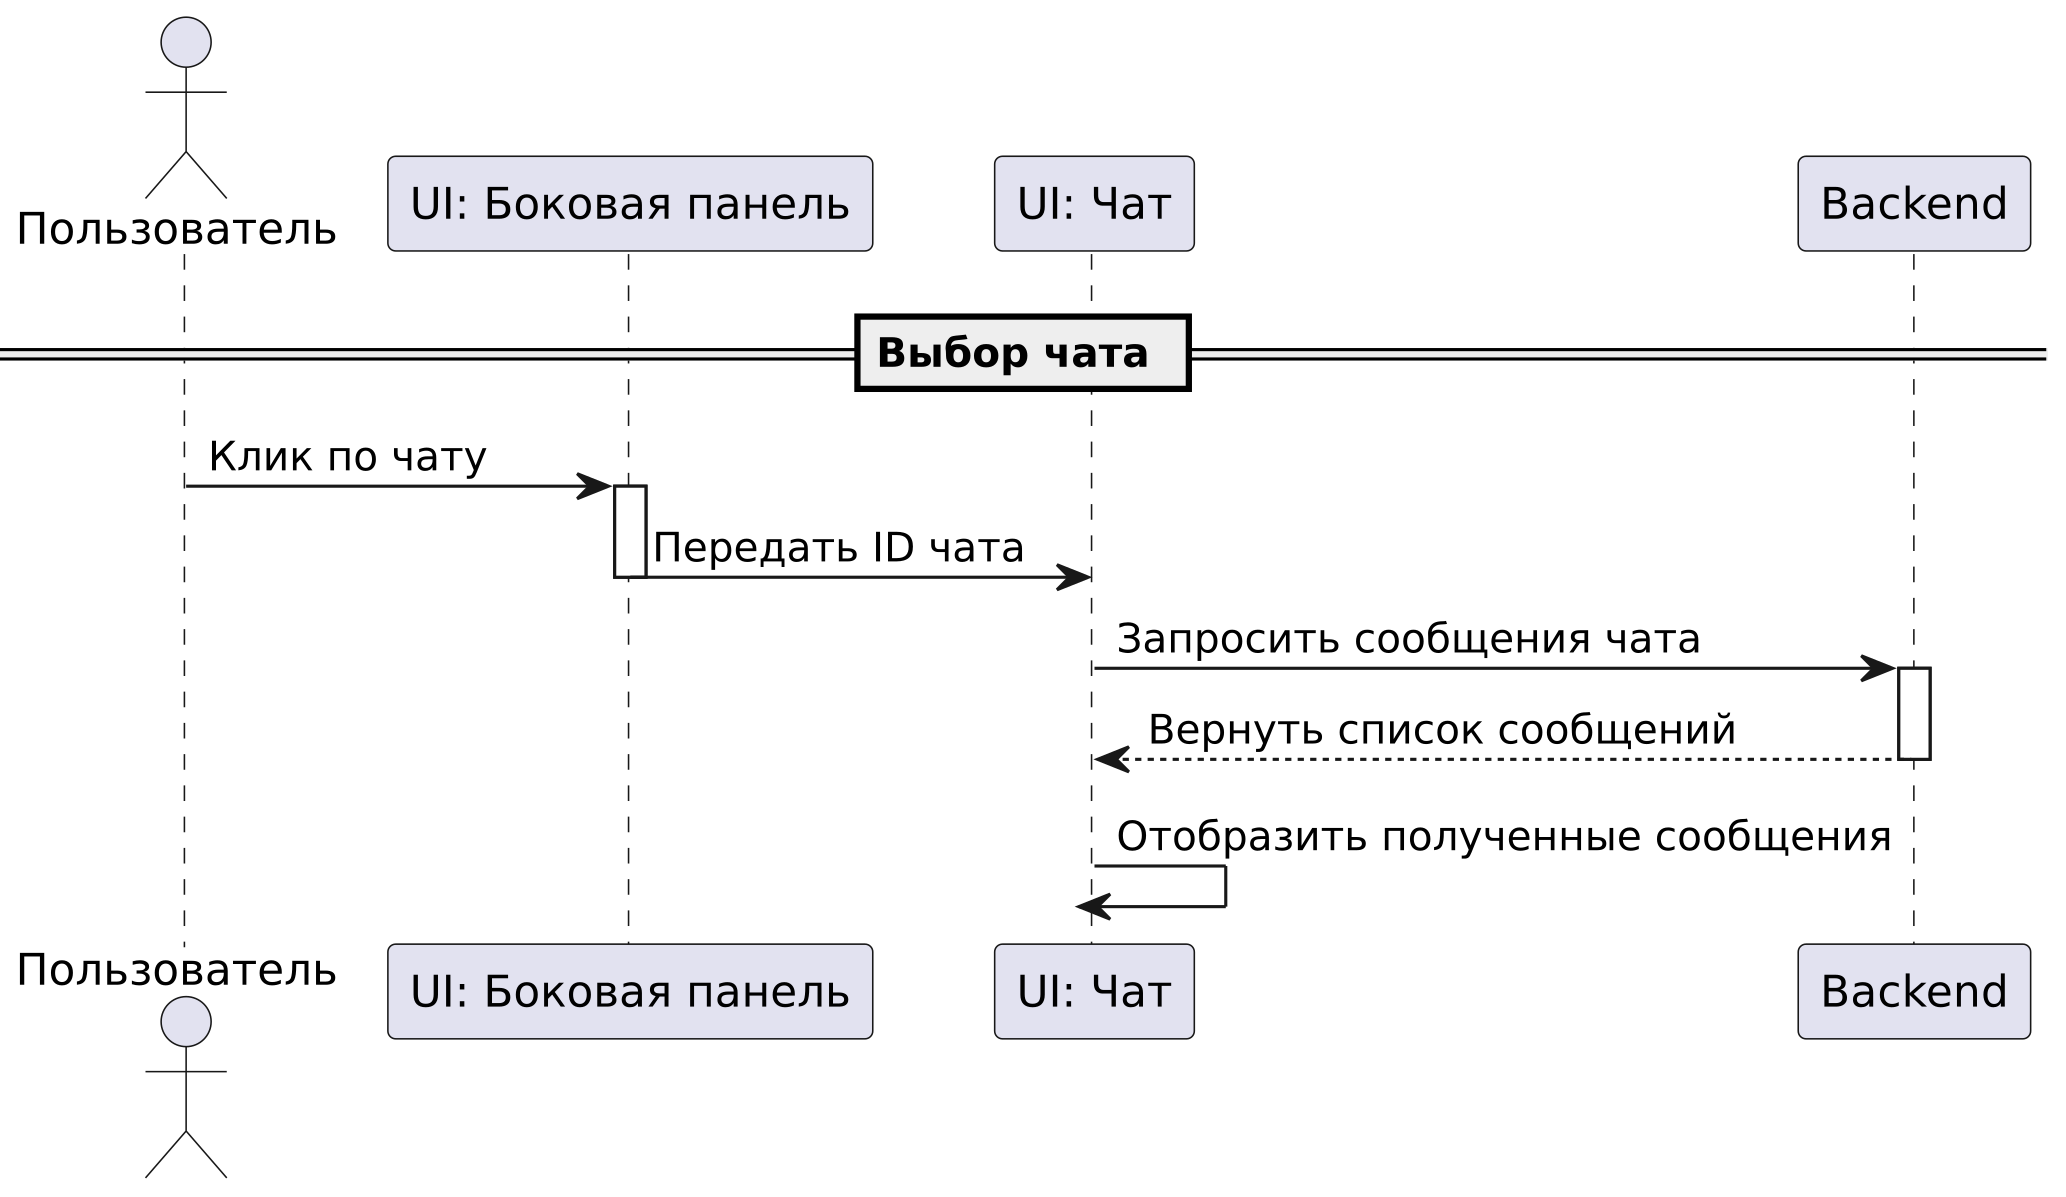
\includegraphics[width=0.95\linewidth]{static/ChatInteractionDiagram.png} \\
        \small Открытие и отображение списка чатов
    \end{column}
\end{columns}
\end{frame}

\begin{frame}{Диаграммы отправки и получения сообщений}
\vspace{0.5em}

\begin{columns}
    \begin{column}{0.5\textwidth}
        \centering
        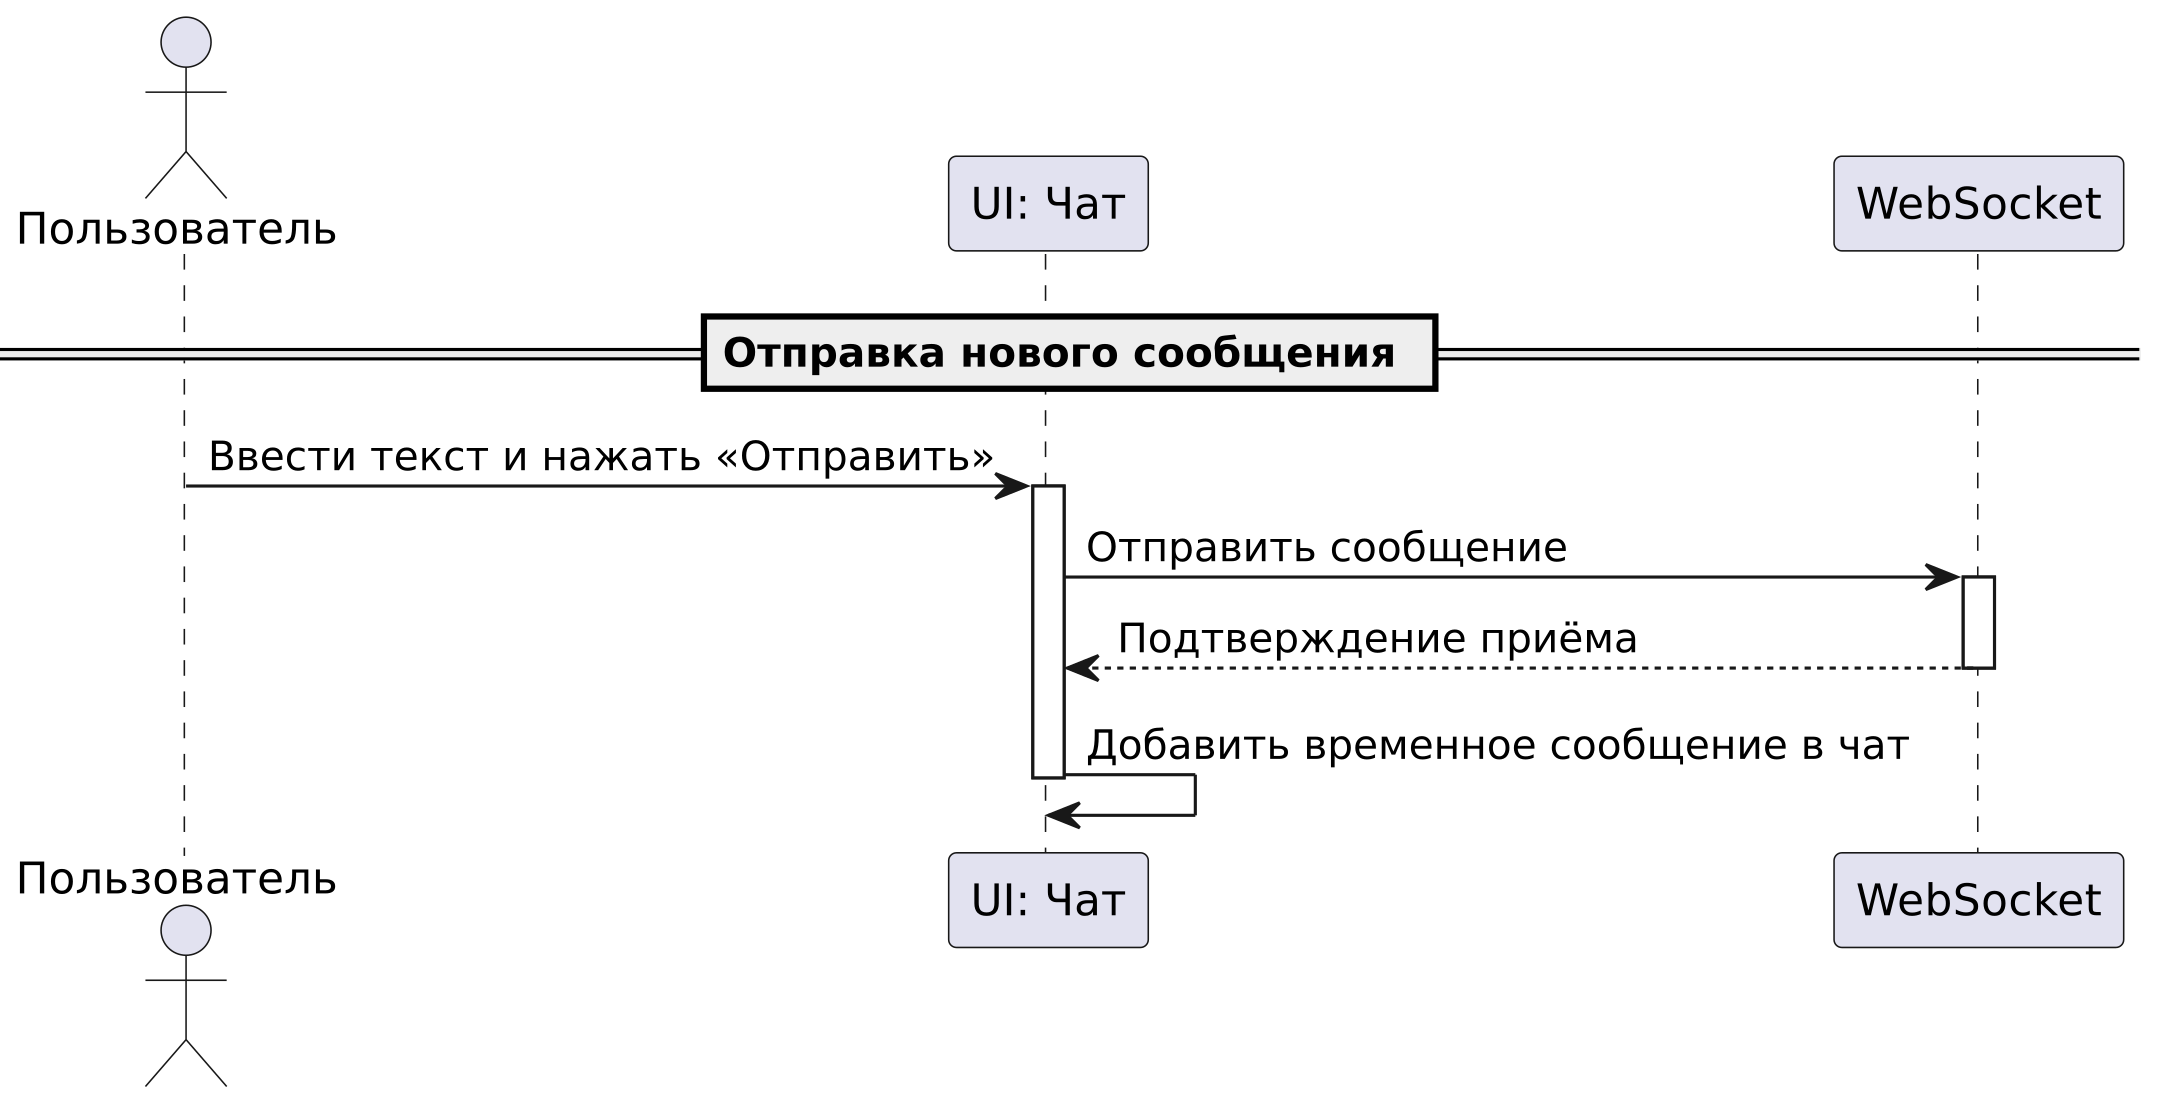
\includegraphics[width=0.95\linewidth]{static/MessageSendDiagram.png} \\
        \small Отправка сообщения пользователем
    \end{column}
    \begin{column}{0.5\textwidth}
        \centering
        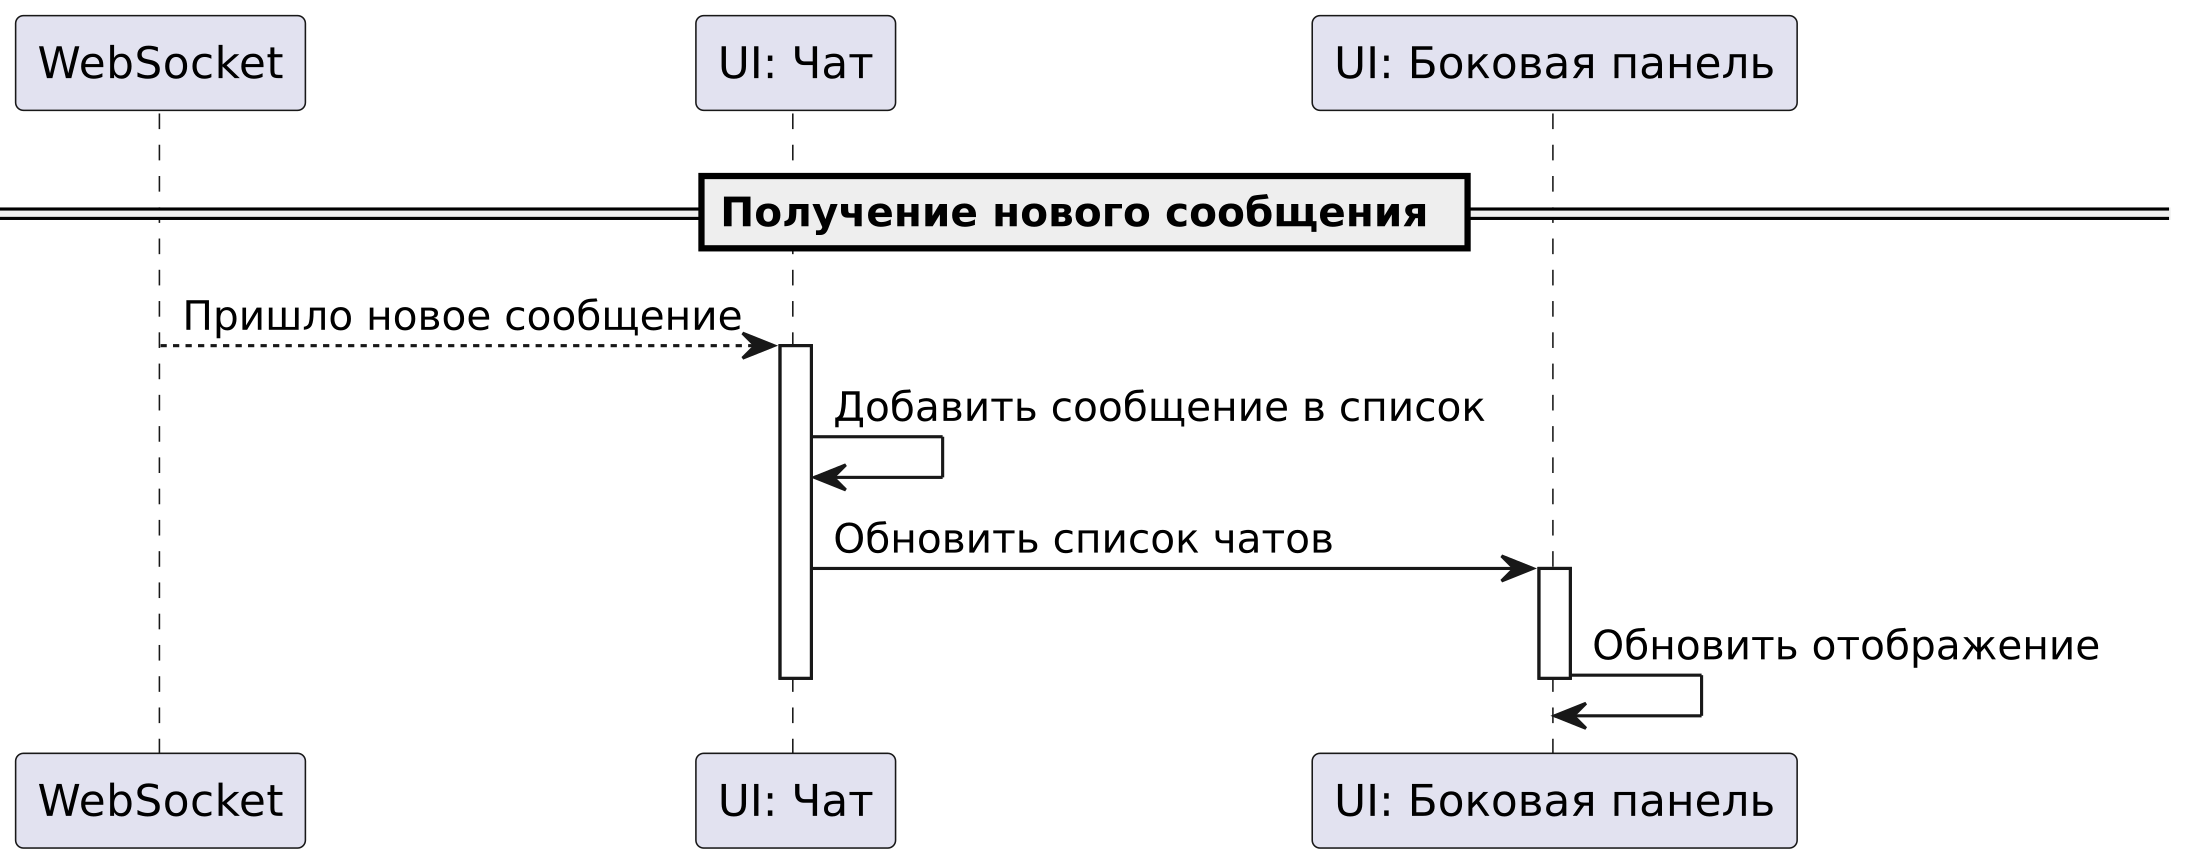
\includegraphics[width=0.95\linewidth]{static/MessageReceiveDiagram.png} \\
        \small Получение сообщения получателем
    \end{column}
\end{columns}
\end{frame}

%\begin{frame}{Диаграммы редактирования и чтения сообщений}
%\vspace{0.5em}
%
%\begin{columns}
%    \begin{column}{0.5\textwidth}
%        \centering
%        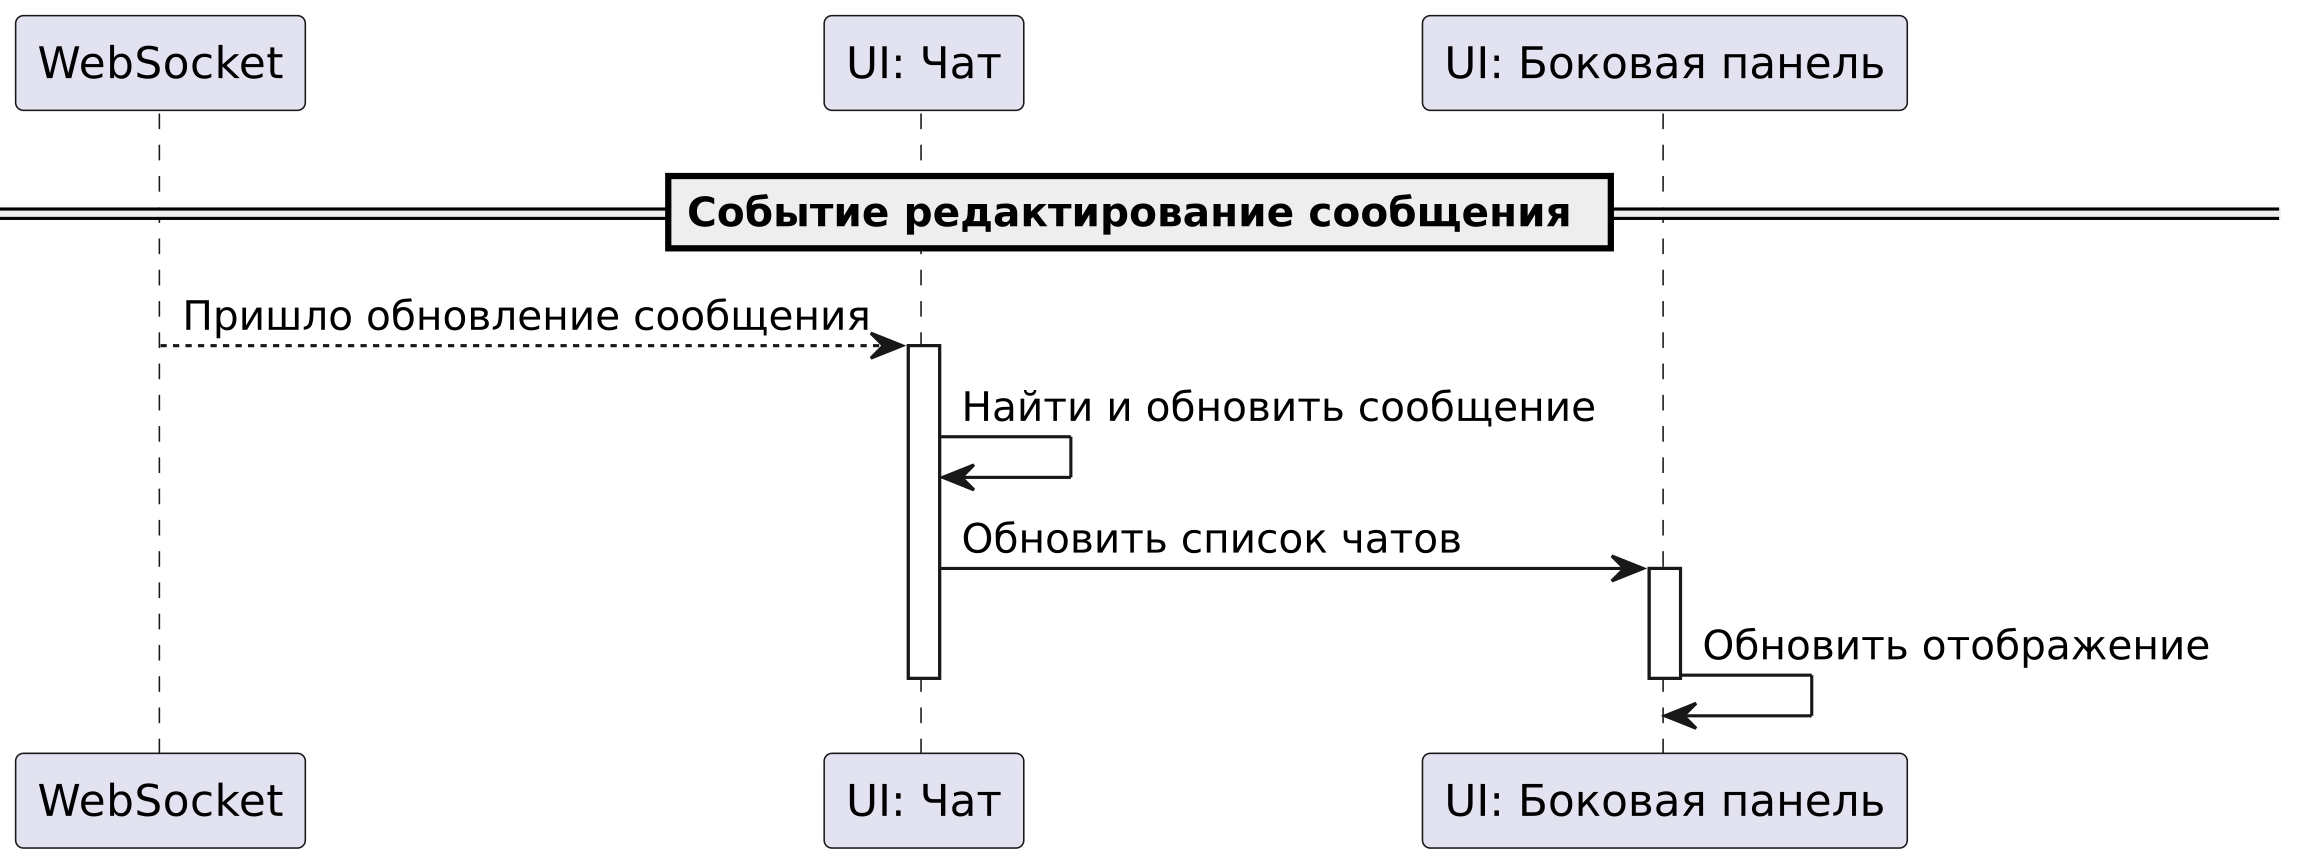
\includegraphics[width=0.95\linewidth]{static/MessageEditDiagram.png} \\
%        \small Редактирование уже отправленного сообщения
%    \end{column}
%    \begin{column}{0.5\textwidth}
%        \centering
%        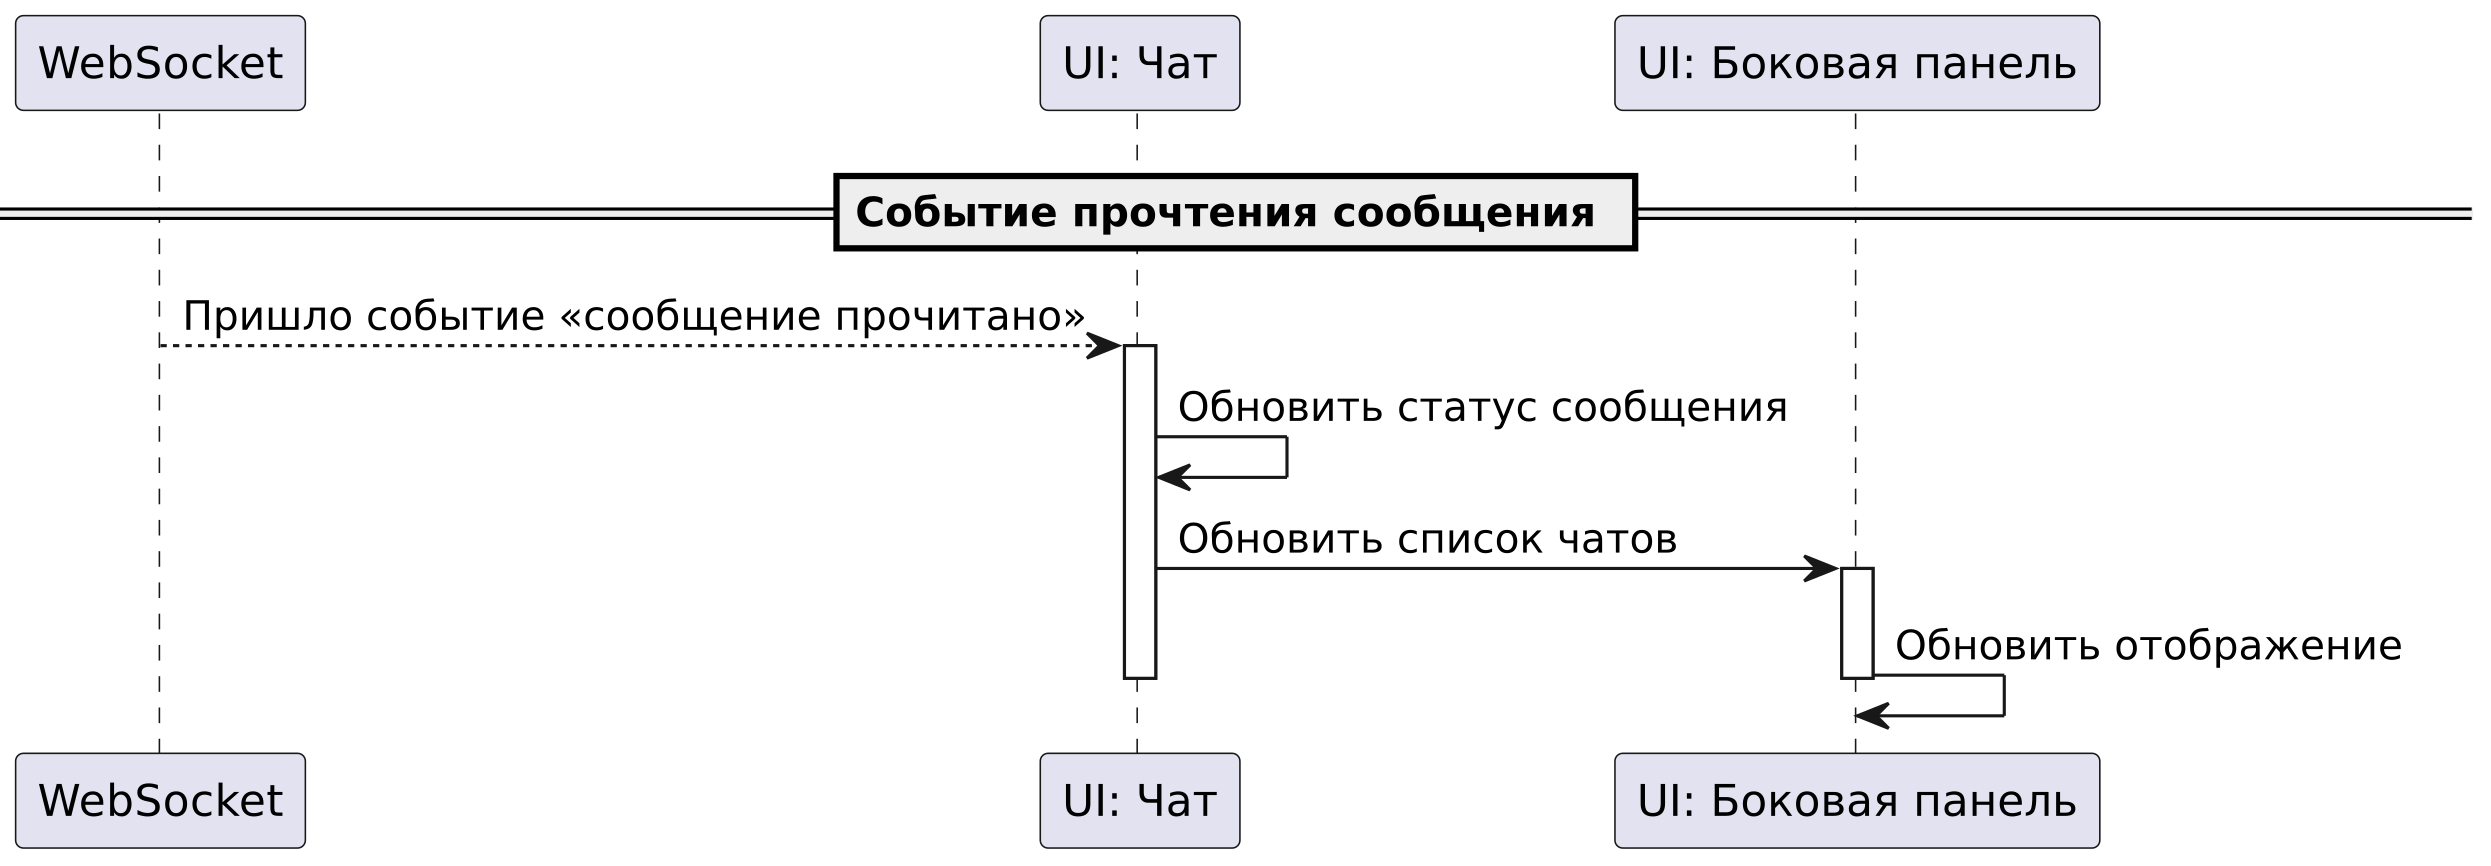
\includegraphics[width=0.95\linewidth]{static/MessageReadDiagram.png} \\
%        \small Отметка о прочтении получателем
%    \end{column}
%\end{columns}
%\end{frame}

\begin{frame}{Переподключение WebSocket: диаграмма последовательности}
\small
\justifying
При истечении срока действия access-токена реализован механизм его автоматического обновления и повторного переподключения WebSocket-соединения.

\vspace{0.5em}

\centering
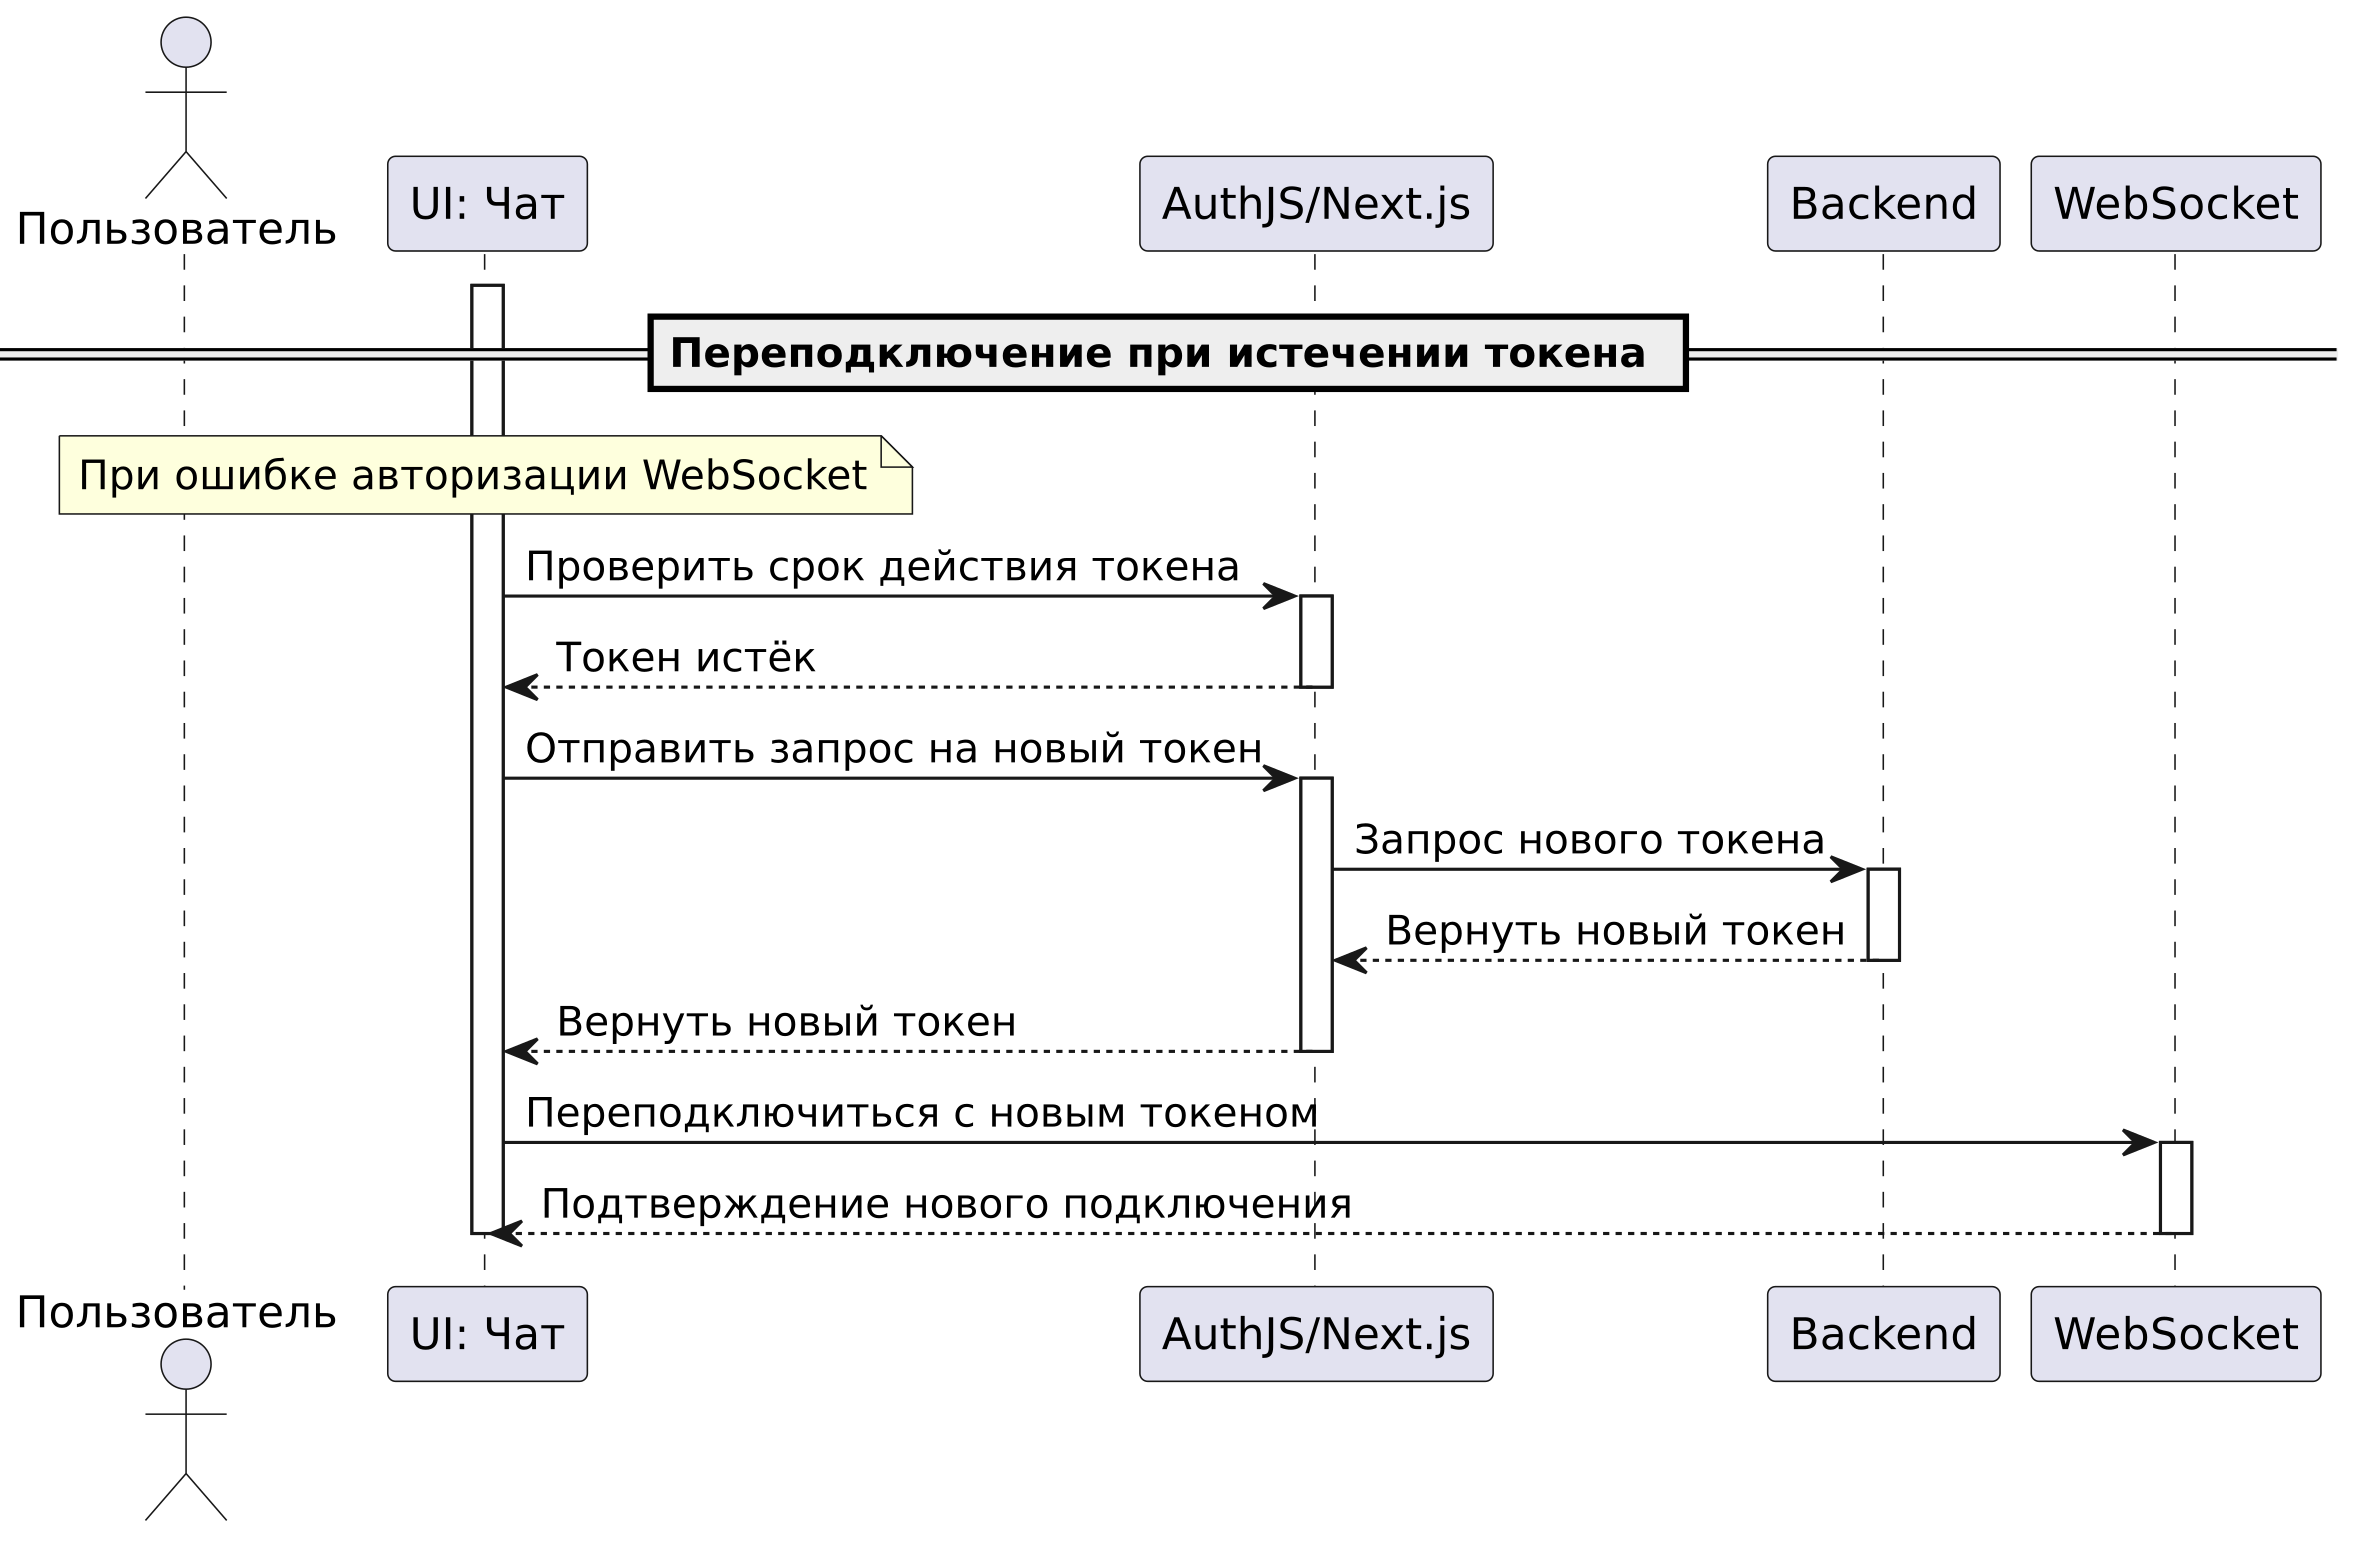
\includegraphics[width=0.7\textwidth]{static/WsReconnectSequence.png}
\end{frame}

\begin{frame}{Интерфейс чата}
\small
\justifying
Пользовательский интерфейс чата предоставляет возможность обмена сообщениями в режиме реального времени.

\vspace{1em}

\centering
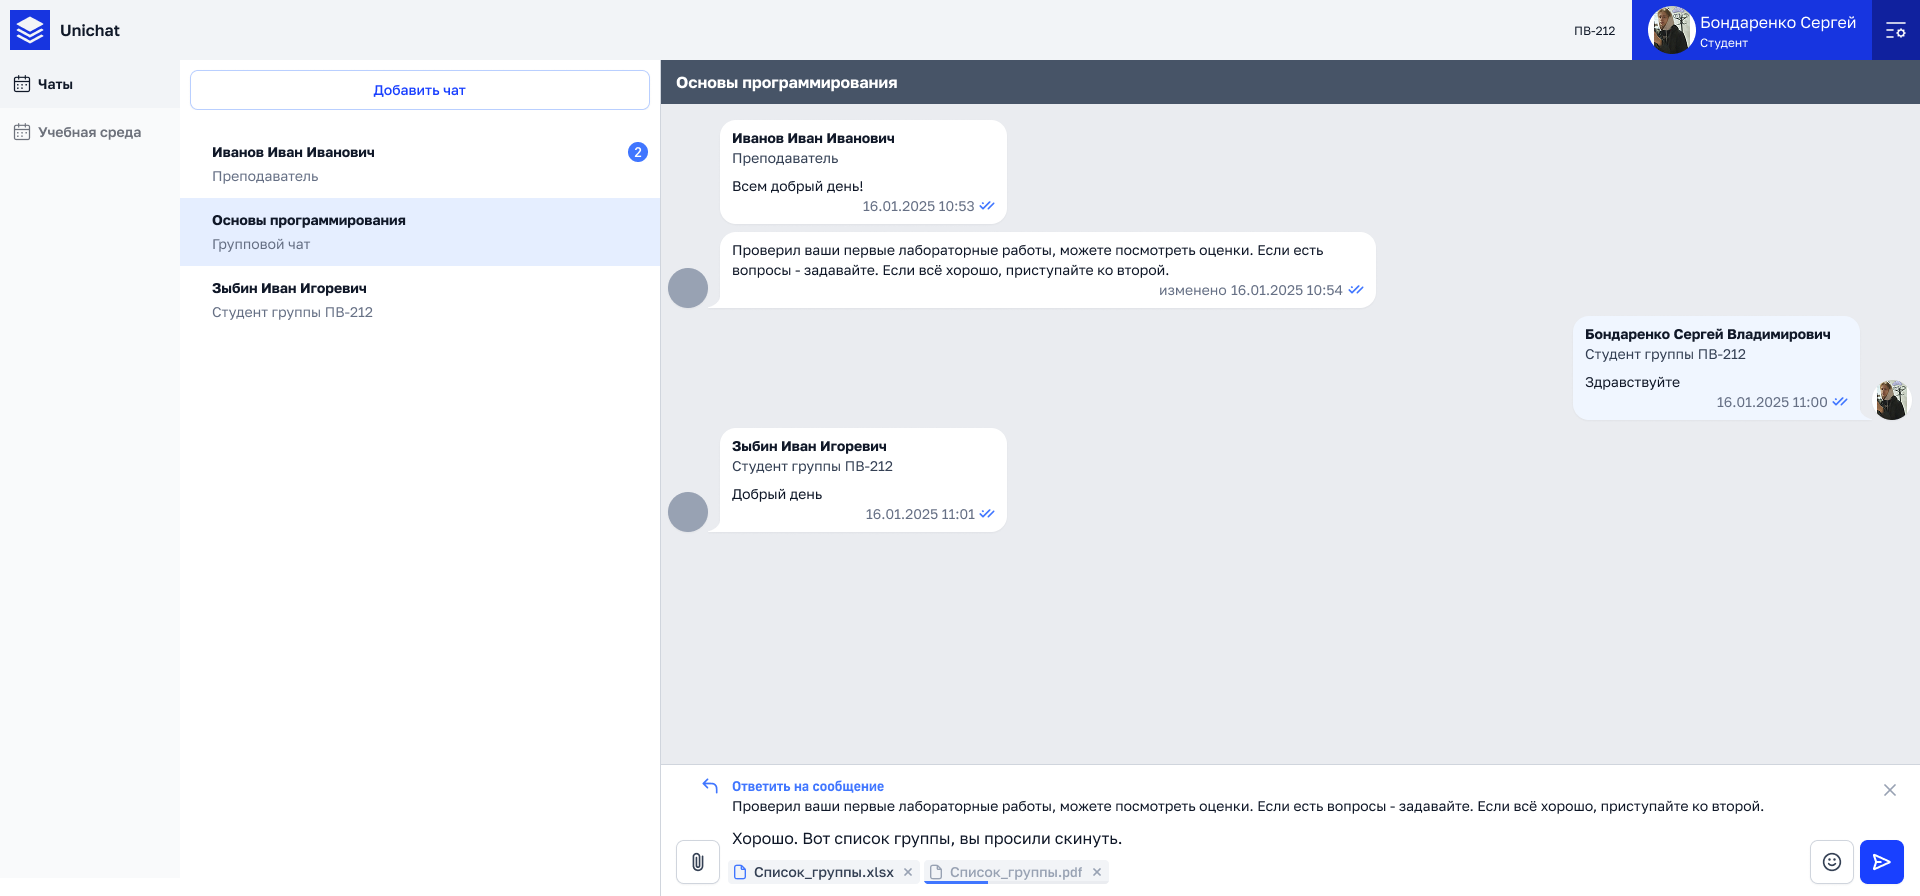
\includegraphics[width=0.85\textwidth]{static/ChatsStudentPage.png}
\end{frame}

%\begin{frame}{Интерфейс создания чатов}
%\small
%\justifying
%Преподаватель может создавать как групповые, так и личные чаты со студентами и коллегами. Студентам доступно только создание личных чатов с преподавателями и студентами.
%
%\vspace{1em}
%
%\begin{columns}
%  \begin{column}{0.5\textwidth}
%    \centering
%    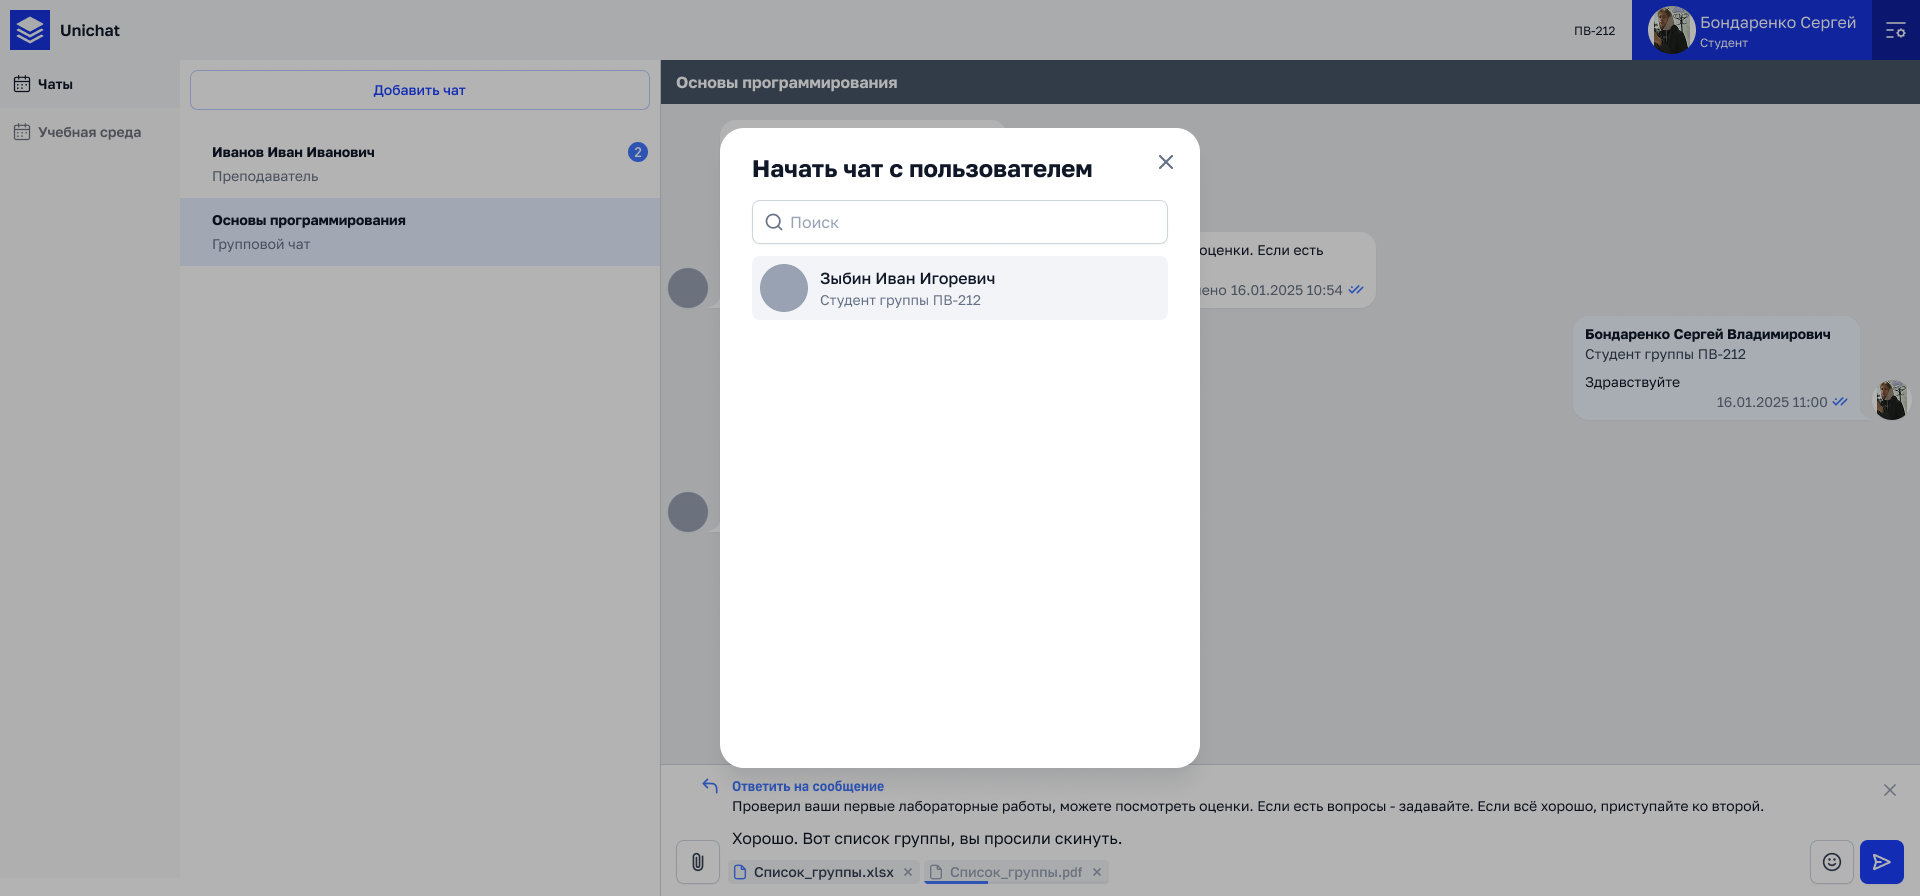
\includegraphics[width=0.95\linewidth]{static/ChatsStudentCreateChat.png} \\
%    \small Личный чат
%  \end{column}
%  \begin{column}{0.5\textwidth}
%    \centering
%    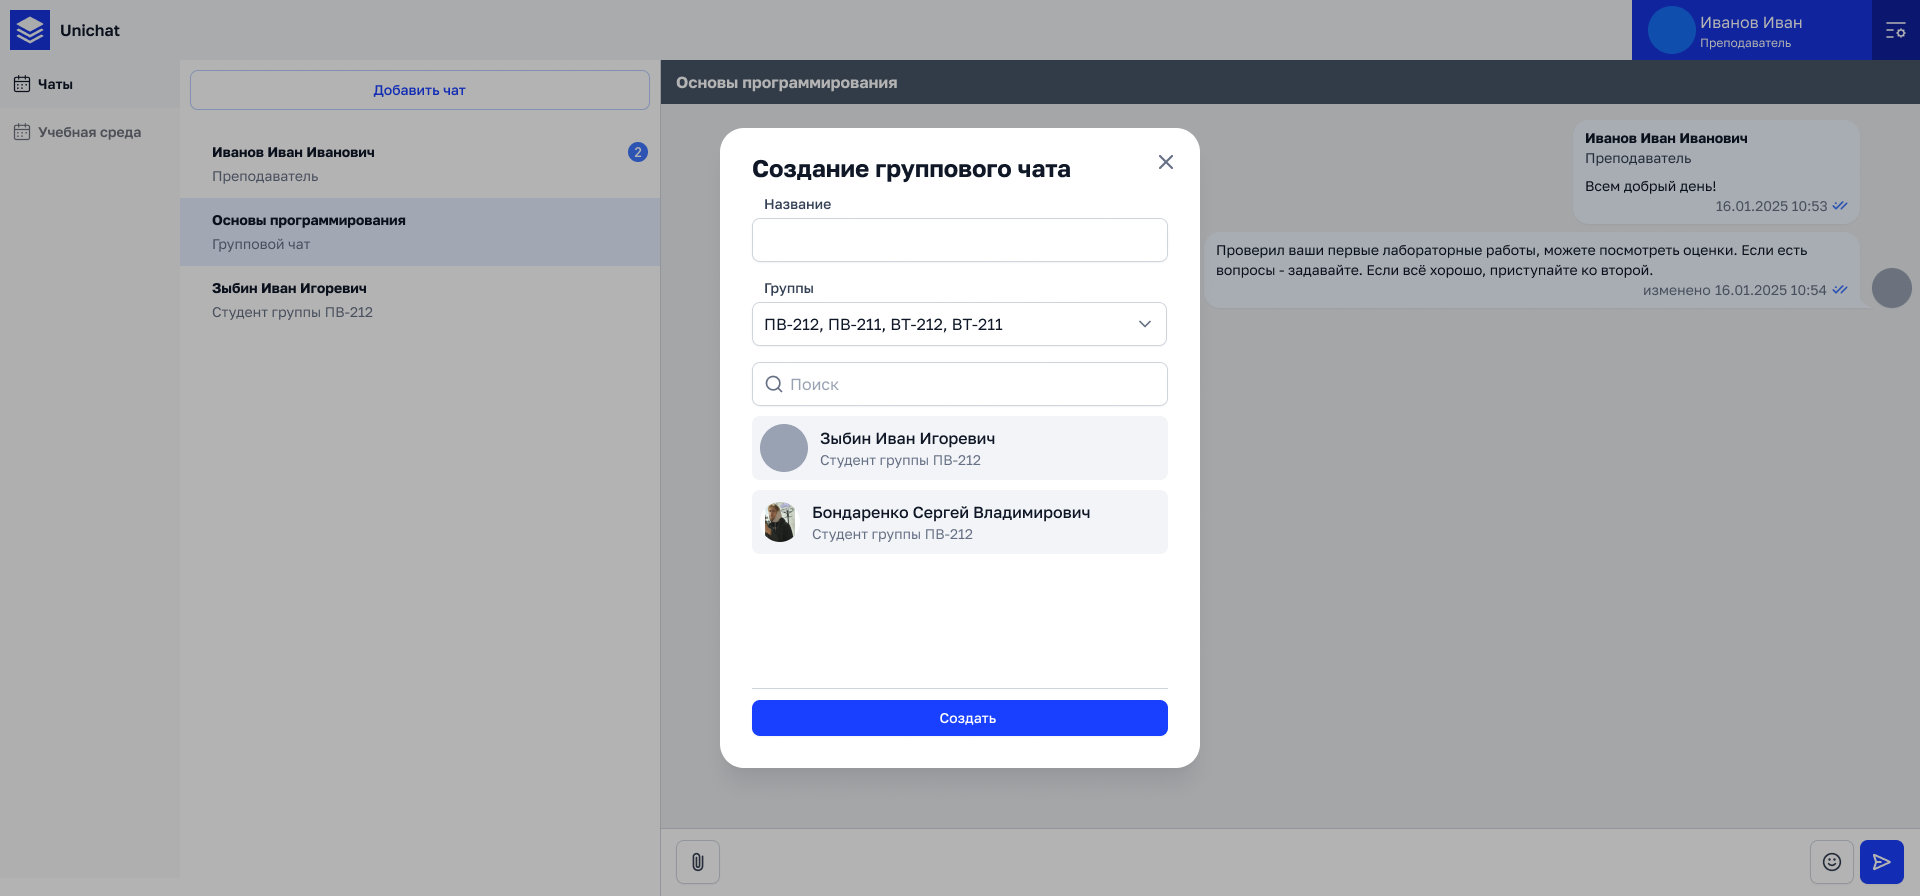
\includegraphics[width=0.95\linewidth]{static/ChatsTeacherCreateGroupChat.png} \\
%    \small Групповой чат
%  \end{column}
%\end{columns}
%\end{frame}

\begin{frame}{Результаты выполнения тестов}
\small
\justifying
В ходе работы была протестирована сложная бизнес-логика Web-приложения. Также проведено тестирование собственной UI-библиотеки.

\vspace{1em}

\begin{columns}
  \begin{column}{0.48\textwidth}
    \centering
    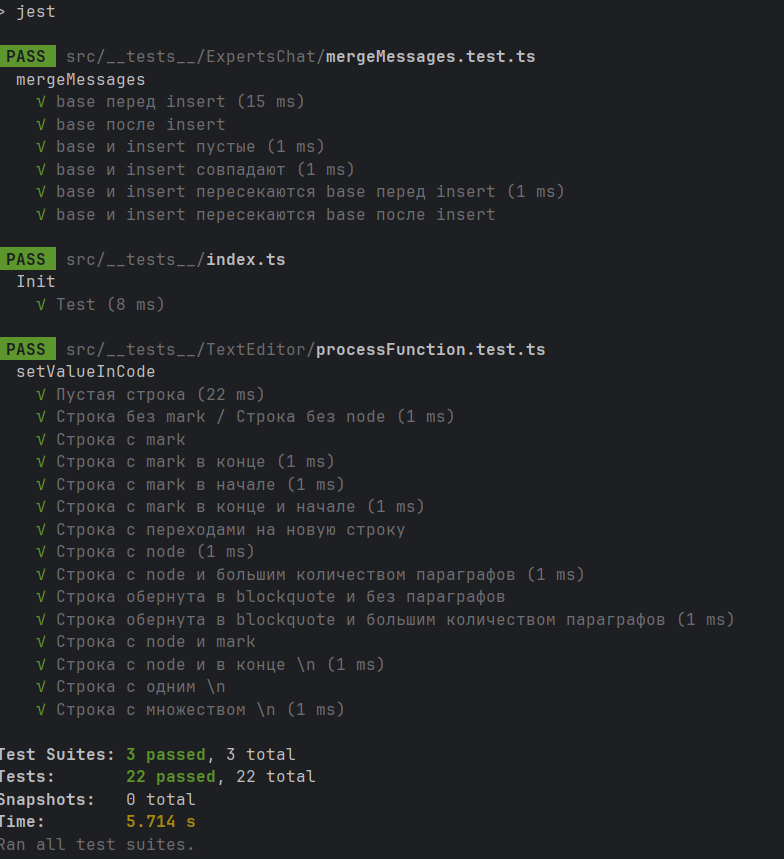
\includegraphics[width=0.8\linewidth]{static/ProjectTests.png} \\
    \small Результаты в Web-приложении
  \end{column}
  \begin{column}{0.48\textwidth}
    \centering
    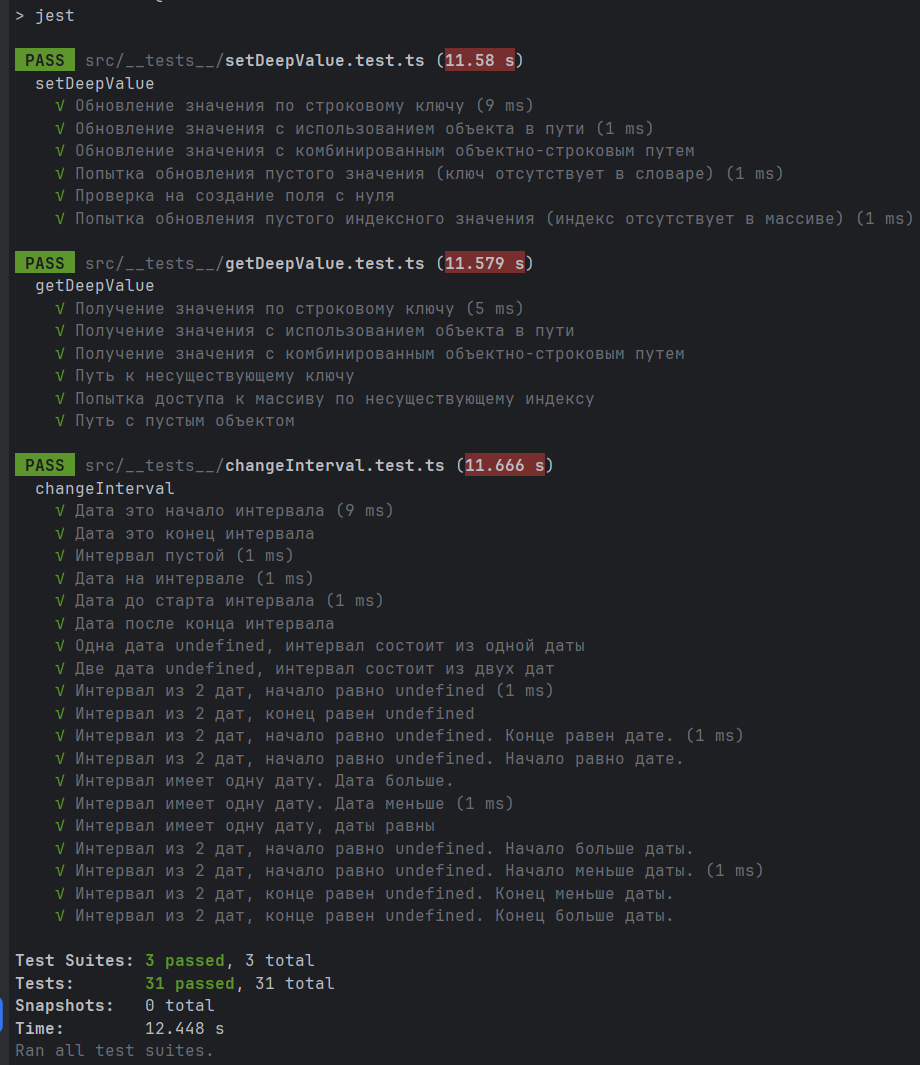
\includegraphics[width=0.8\linewidth]{static/LibTests.png} \\
    \small Результаты в UI-библиотеке
  \end{column}
\end{columns}
\end{frame}

\begin{frame}{Заключение}
\small
В ходе выполнения выпускной квалификационной работы были успешно решены поставленные задачи:

\begin{itemize}
  \item Проведён анализ существующих образовательных приложений и решений для автоматизированной проверки кода;
  \item Разработана архитектура front-end части Web–приложения с применением Feature-Sliced Design и современных паттернов проектирования;
  \item Разработан удобный пользовательский интерфейс для студентов и преподавателей;
  \item Реализованы модули аутентификации, управления заданиями, чатами, а также внедрён механизм обмена сообщениями в реальном времени через WebSocket с обработкой переподключения и синхронизацией состояния;
  \item Реализована интеграция с AI для автоматизированной проверки решений;
  \item Проведено тестирование бизнес-логики Web–приложения, подтверждающее корректность работы основных функций.
\end{itemize}
\end{frame}


\begin{frame}{Интерфейс создания приглашения пользователей}
\vspace{0.5em}

\begin{columns}
    \begin{column}{0.5\textwidth}
        \centering
        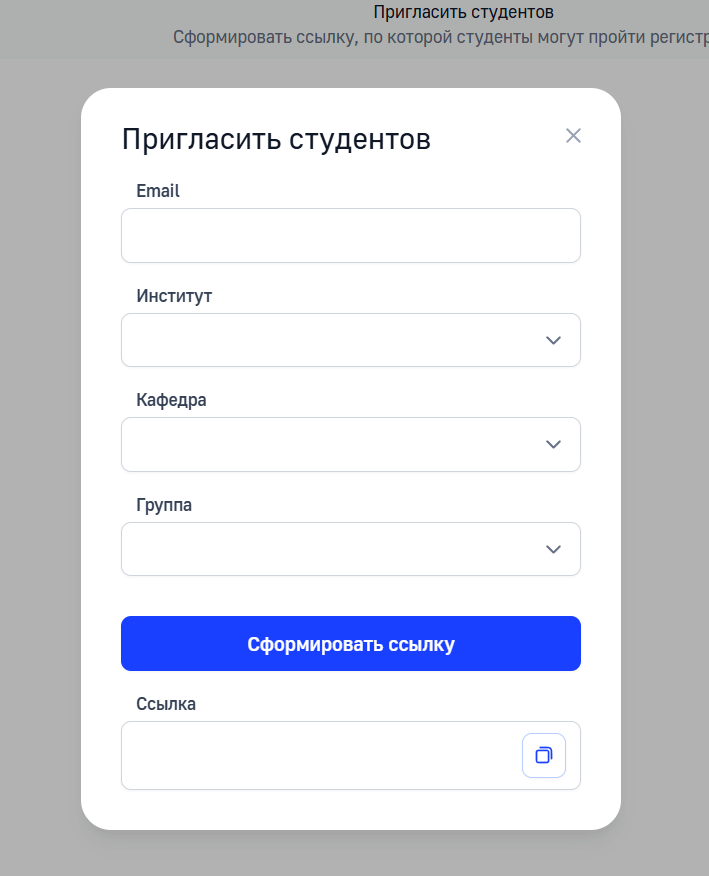
\includegraphics[width=0.95\linewidth]{static/InviteStudentPage.png} \\
        \small Форма приглашения студента
    \end{column}
    \begin{column}{0.5\textwidth}
        \centering
        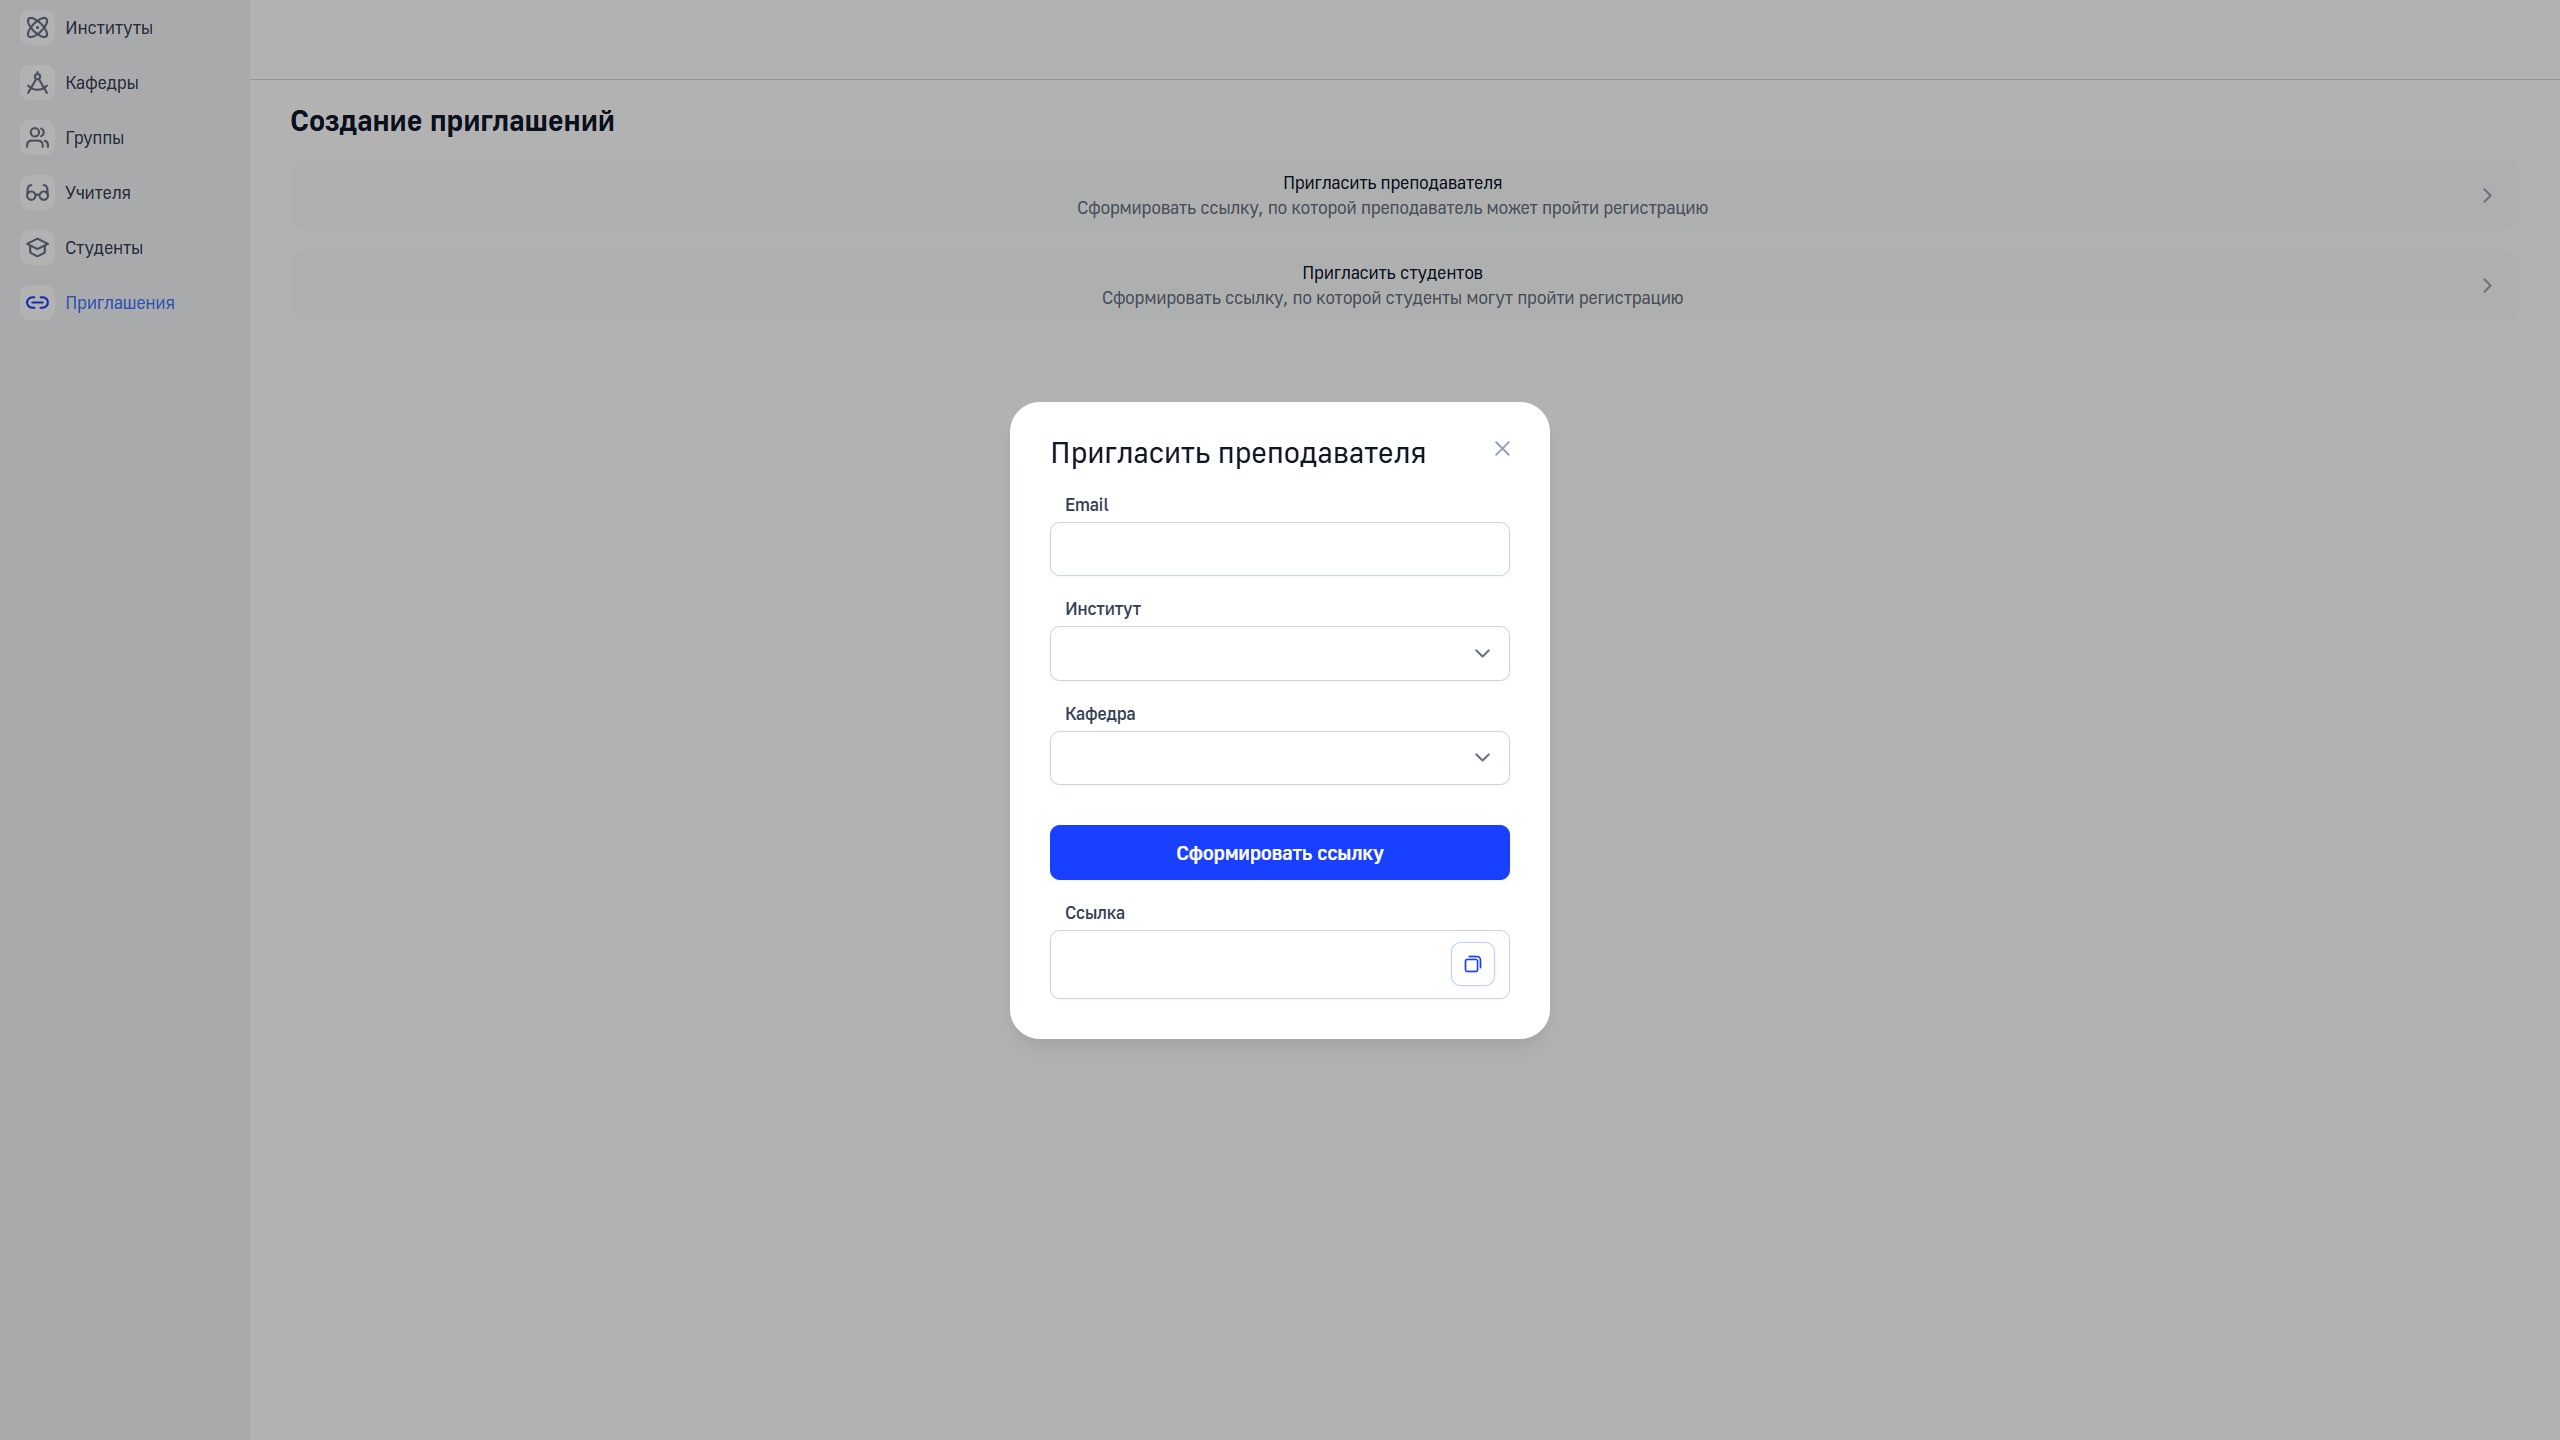
\includegraphics[width=0.95\linewidth]{static/InviteTeacherPage.png} \\
        \small Форма приглашения преподавателя
    \end{column}
\end{columns}
\end{frame}


\begin{frame}{Интерфейс Регистрации}
\begin{columns}
    \begin{column}{0.45\textwidth}
        \centering
        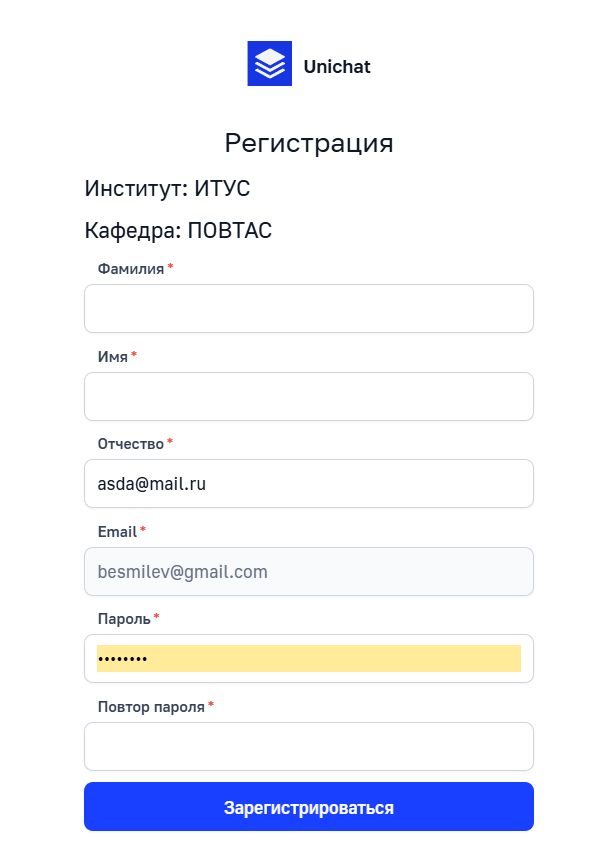
\includegraphics[height=5cm]{static/RegTeacherPage.png} \\
        \small Регистрация преподавателя
    \end{column}
    \begin{column}{0.45\textwidth}
        \centering
        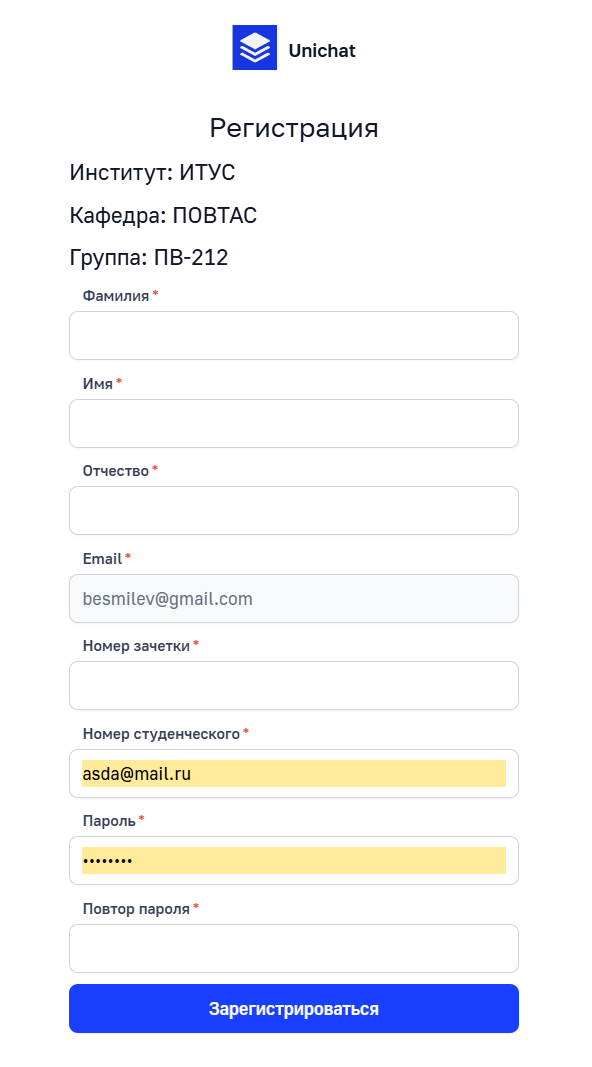
\includegraphics[height=5cm]{static/RegStudentPage.png} \\
        \small Регистрация студента
    \end{column}
\end{columns}
\end{frame}


\begin{frame}{Интерфейс списка и просмотра заданий}
\vspace{0.5em}

\begin{columns}
    \begin{column}{0.5\textwidth}
        \centering
        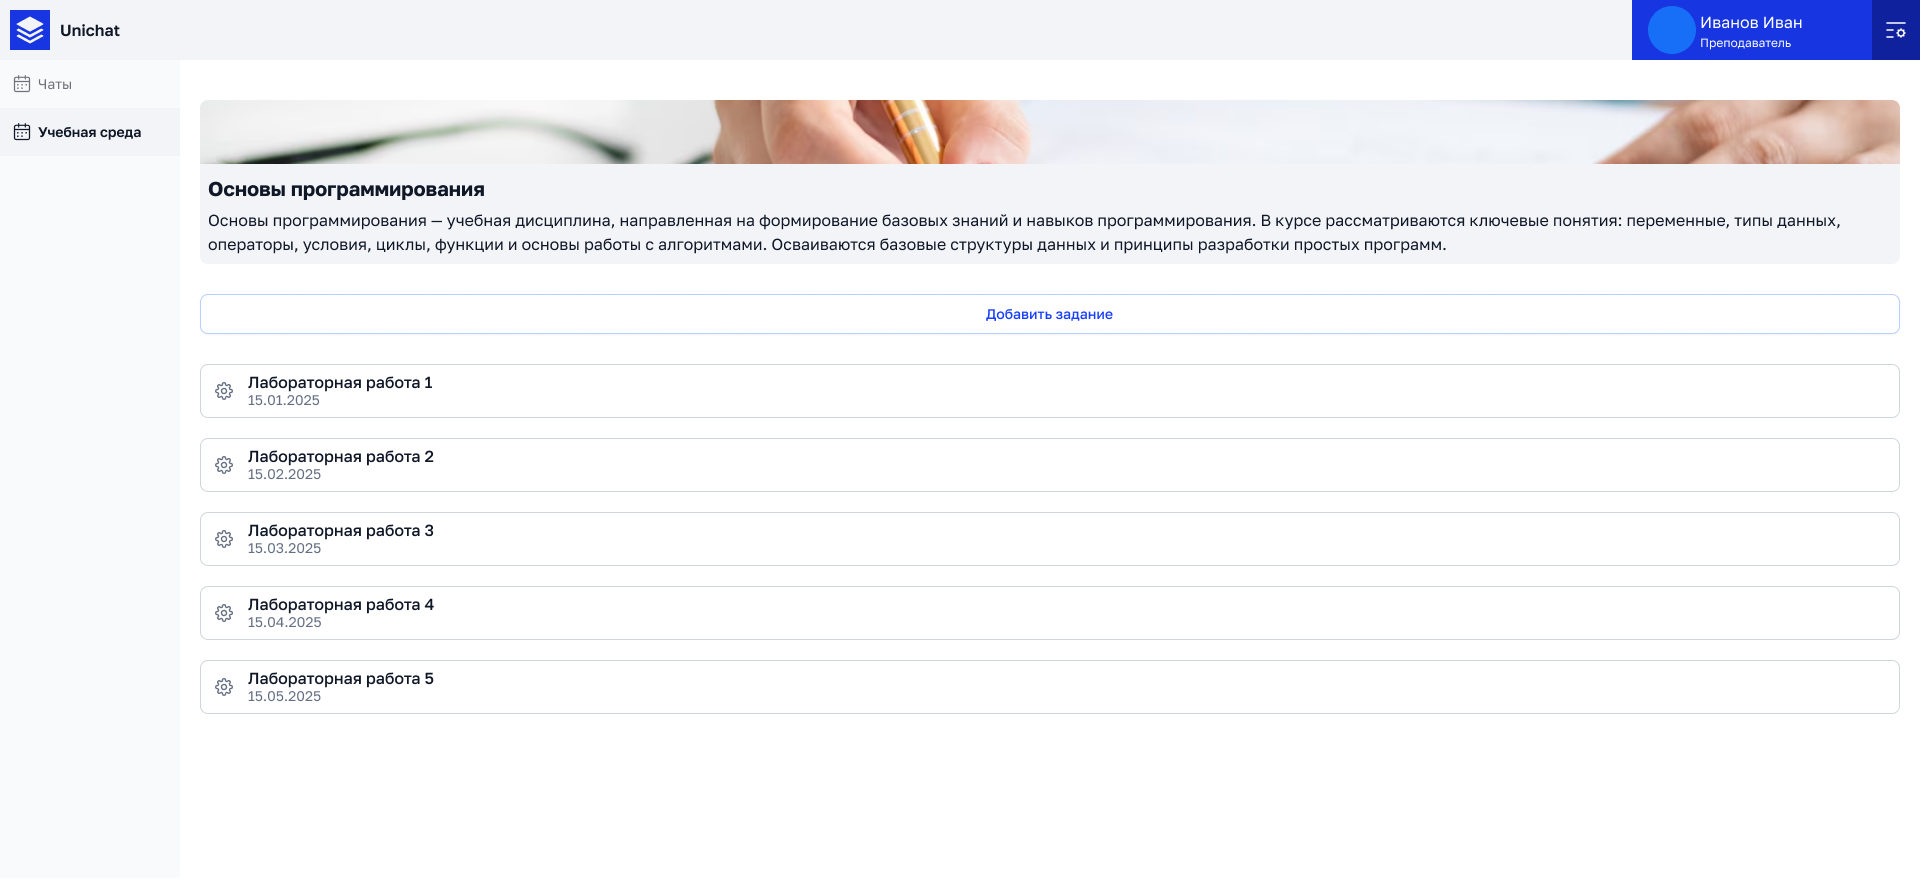
\includegraphics[width=0.9\linewidth]{static/TaskListTeacher.png} \\
        \small Список заданий

        \vspace{1em}

        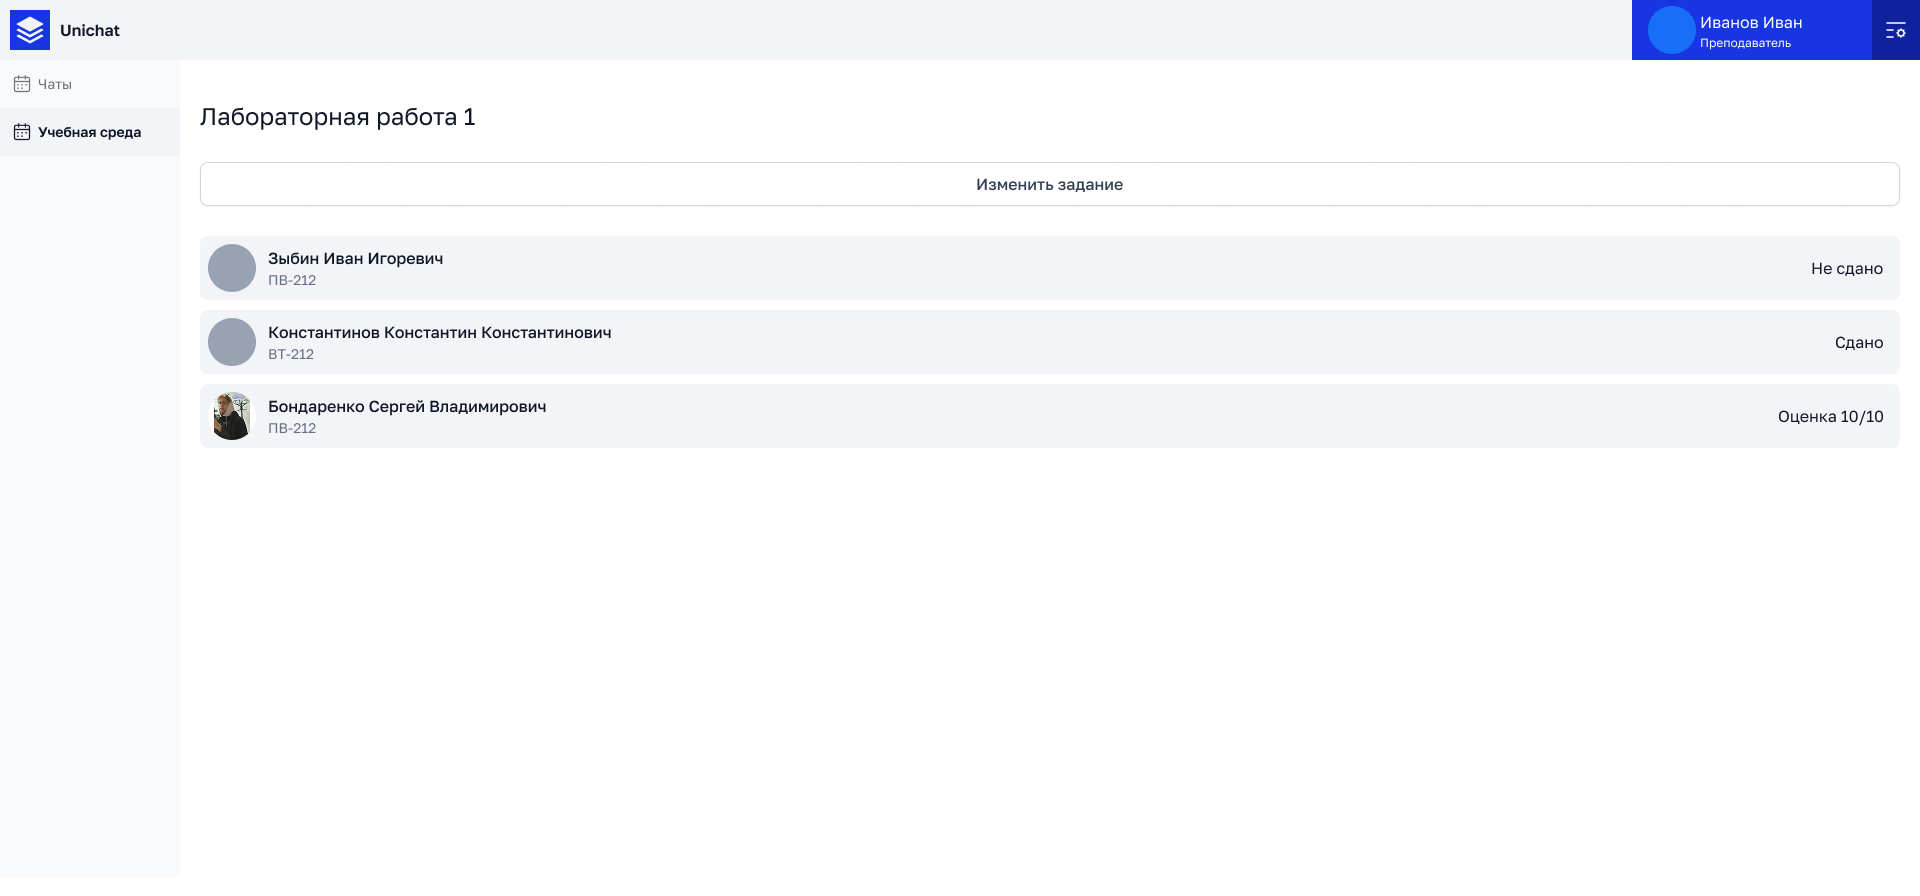
\includegraphics[width=0.9\linewidth]{static/TaskTeacherDetail.png} \\
        \small Просмотр задания преподавателем
    \end{column}
    \begin{column}{0.5\textwidth}
        \centering
        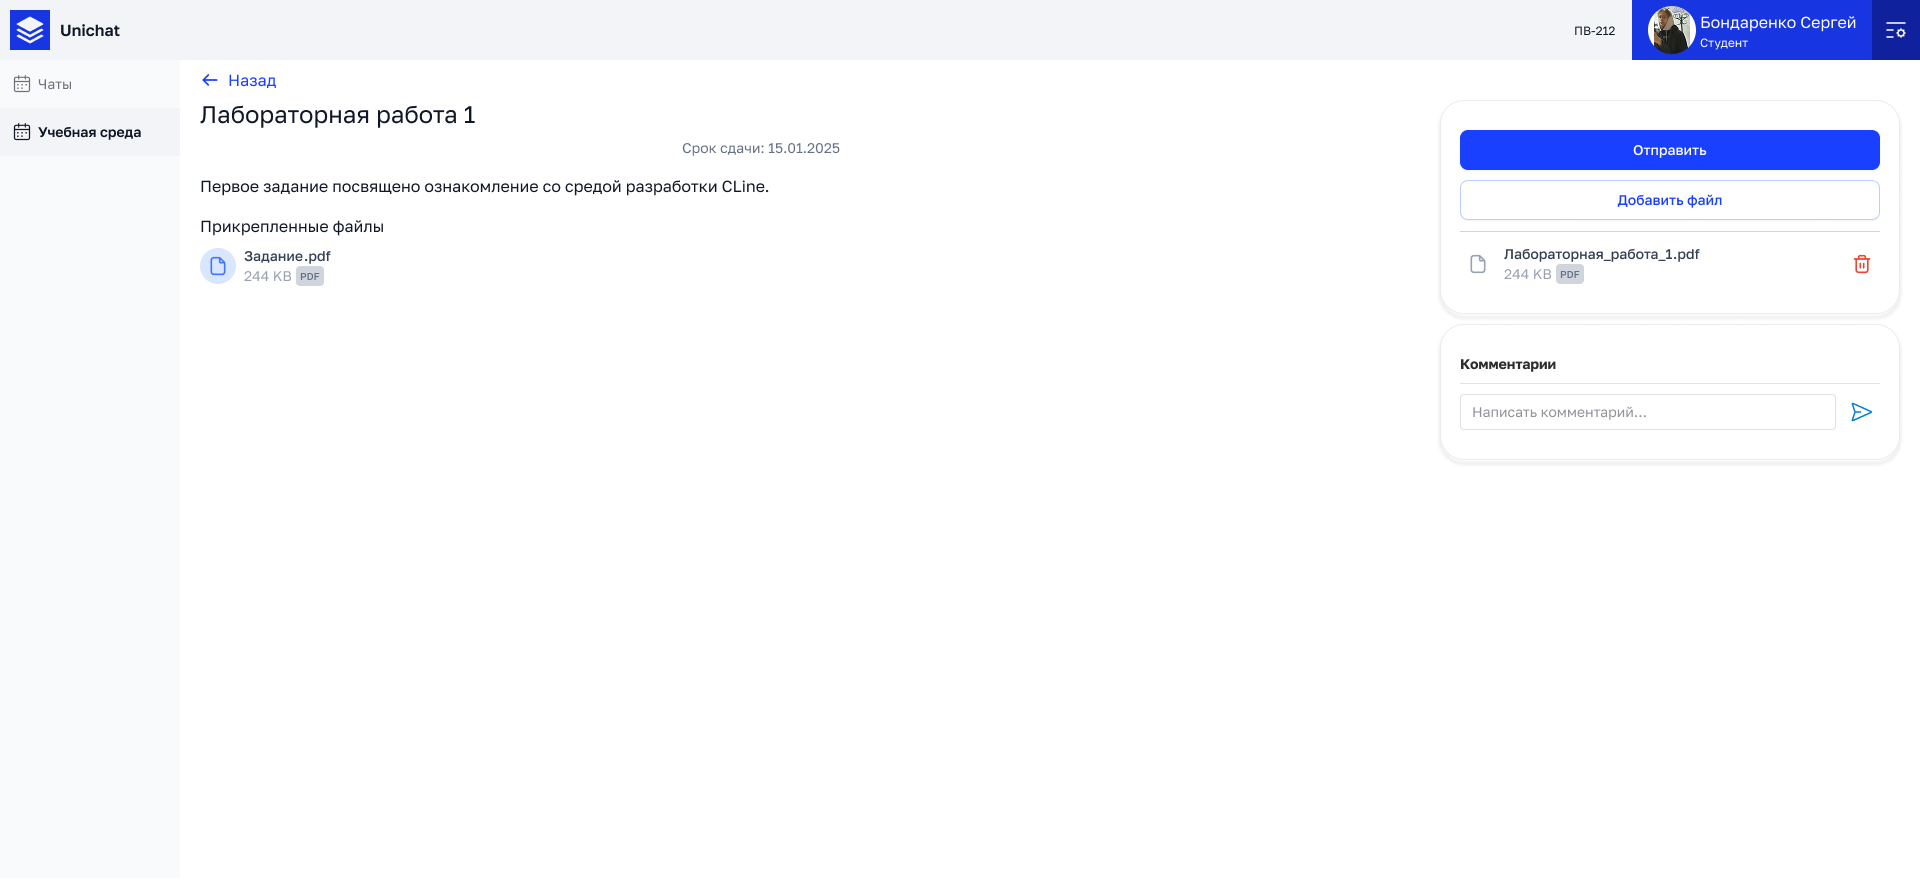
\includegraphics[width=0.95\linewidth]{static/TaskStudentNotSend.png} \\
        \small Просмотр задания студентом
    \end{column}
\end{columns}
\end{frame}

\end{document}
